\clearpage
\subsection{MC Closure Test for the Object Replacement Method Estimating the Soft-Lepton Regions} \label{sec::App::objRep_closure_softLep}
While the closure test estimating hard lepton regions are shown in Sec. \ref{sec::BGestimation::objRep::mcClosure}, this section presents the case of soft-lepton regions. 
Figure \ref{fig::ObjReplace::mcClosure_softLep_MisLep_el}, \ref{fig::ObjReplace::mcClosure_softLep_MisLep_mu} and \ref{fig::ObjReplace::mcClosure_softLep_TauRep_emu} respectively illustrate the closure of missing-electron, missing-muon replacement, and the tau replacement in which the tag lepton is soft ($\pt\in[6,35]\gev$). The common 2LCR selection is used as the case in Sec. \ref{sec::BGestimation::objRep::mcClosure}. Though it is somtimes a bit subtle due to the limited MC statistics, good agreement is seen in general.

% ---------- mcClosure::plot::softLep
%%%%% METHNAME %%%%%%%%%%%%%%%%%%%%%%%%%%
\begin{figure}[h]
  \centering
    \subfig{0.28}{figures/BGestimation/ObjReplacement/mcClosure_softlep/MisLep_el_softLep/MisLep_el_jet1Pt__trMode4_NoSys_softLep.pdf}{$\pt$ of the leading jet}
    \subfig{0.28}{figures/BGestimation/ObjReplacement/mcClosure_softlep/MisLep_el_softLep/MisLep_el_meffInc30__trMode4_NoSys_softLep.pdf}{$\meffInc$}
    \subfig{0.28}{figures/BGestimation/ObjReplacement/mcClosure_softlep/MisLep_el_softLep/MisLep_el_met__trMode4_NoSys_softLep.pdf}{$\met$}
    \subfig{0.28}{figures/BGestimation/ObjReplacement/mcClosure_softlep/MisLep_el_softLep/MisLep_el_mt__trMode4_NoSys_softLep.pdf}{$\mt$}
    \subfig{0.28}{figures/BGestimation/ObjReplacement/mcClosure_softlep/MisLep_el_softLep/MisLep_el_metOverMeff__trMode4_NoSys_softLep.pdf}{$\met/\meffInc$}
    \subfig{0.28}{figures/BGestimation/ObjReplacement/mcClosure_softlep/MisLep_el_softLep/MisLep_el_LepAplanarity__trMode4_NoSys_softLep.pdf}{Aplanarity}
    \subfig{0.28}{figures/BGestimation/ObjReplacement/mcClosure_softlep/MisLep_el_softLep/MisLep_el_min_dPhi_4j__trMode4_NoSys_softLep.pdf}{$\mindPhiFourJet$}
    \subfig{0.28}{figures/BGestimation/ObjReplacement/mcClosure_softlep/MisLep_el_softLep/MisLep_el_nJet30__trMode4_NoSys_softLep.pdf}{Jet multiplicity}
    \subfig{0.28}{figures/BGestimation/ObjReplacement/mcClosure_softlep/MisLep_el_softLep/MisLep_el_nBJet30__trMode4_NoSys_softLep.pdf}{$b$-jet multiplicity}
    \caption{ MC closure test for \textbf{missing lepton replacement} using $t\bar{t}$ MC sample. Seed events are collected by the use of MET trigger. $p_T<35\gev$ for the leading lepton is required. \textbf{Only electrons in the seed events are replaced}. Red points in the bottom plots show the ratio of integrated yields for the two histograms above the x-position that the point indicates. \label{fig::ObjReplace::mcClosure_softLep_MisLep_el} }
\end{figure}
 %%%%%%%%%%%%%%%%%%%%%%%%%%

%%%%% METHNAME %%%%%%%%%%%%%%%%%%%%%%%%%%
\begin{figure}[h]
  \centering
    \subfigure[]{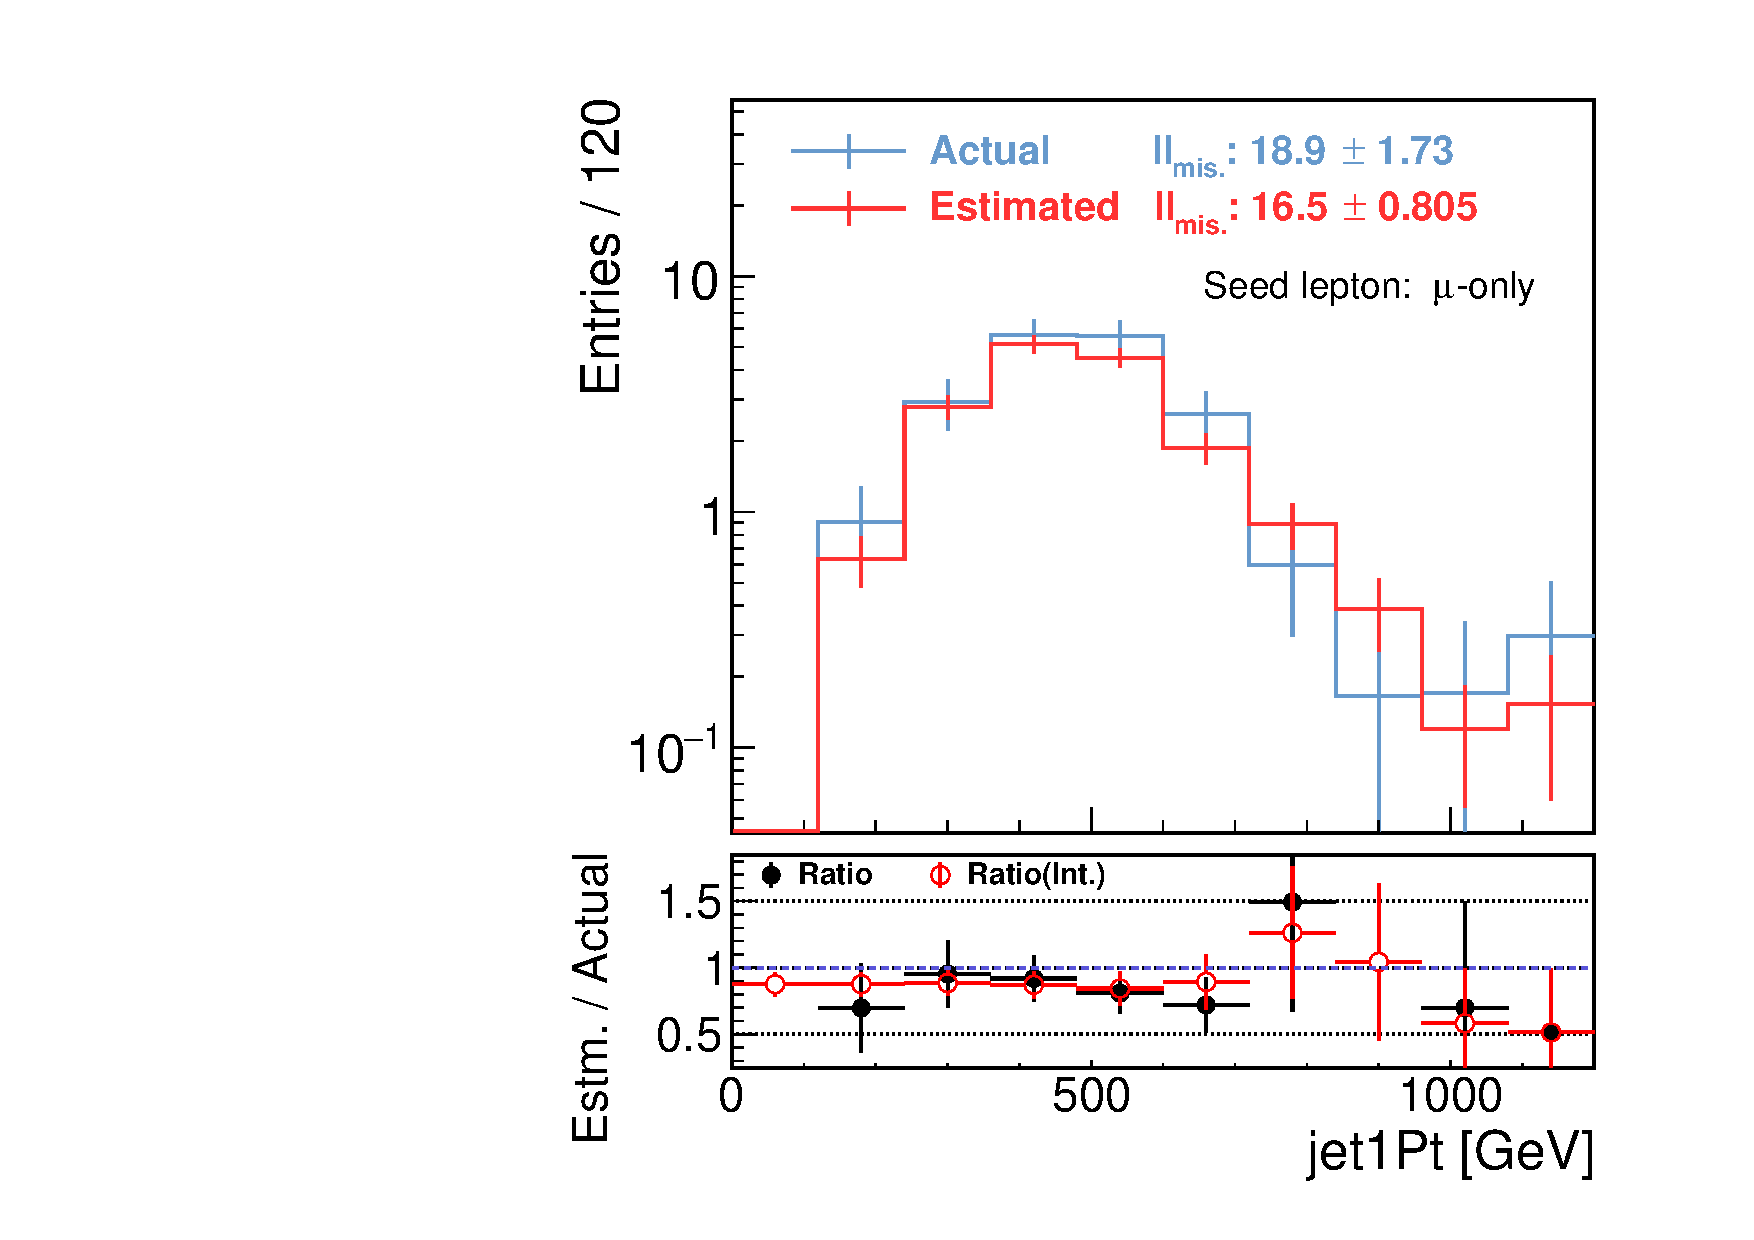
\includegraphics[width=0.32\textwidth]{figures/BGestimation/ObjReplacement/mcClosure_softLep/MisLep_mu_softLep/MisLep_mu_jet1Pt__trMode4_NoSys_softLep.pdf}}
    \subfigure[]{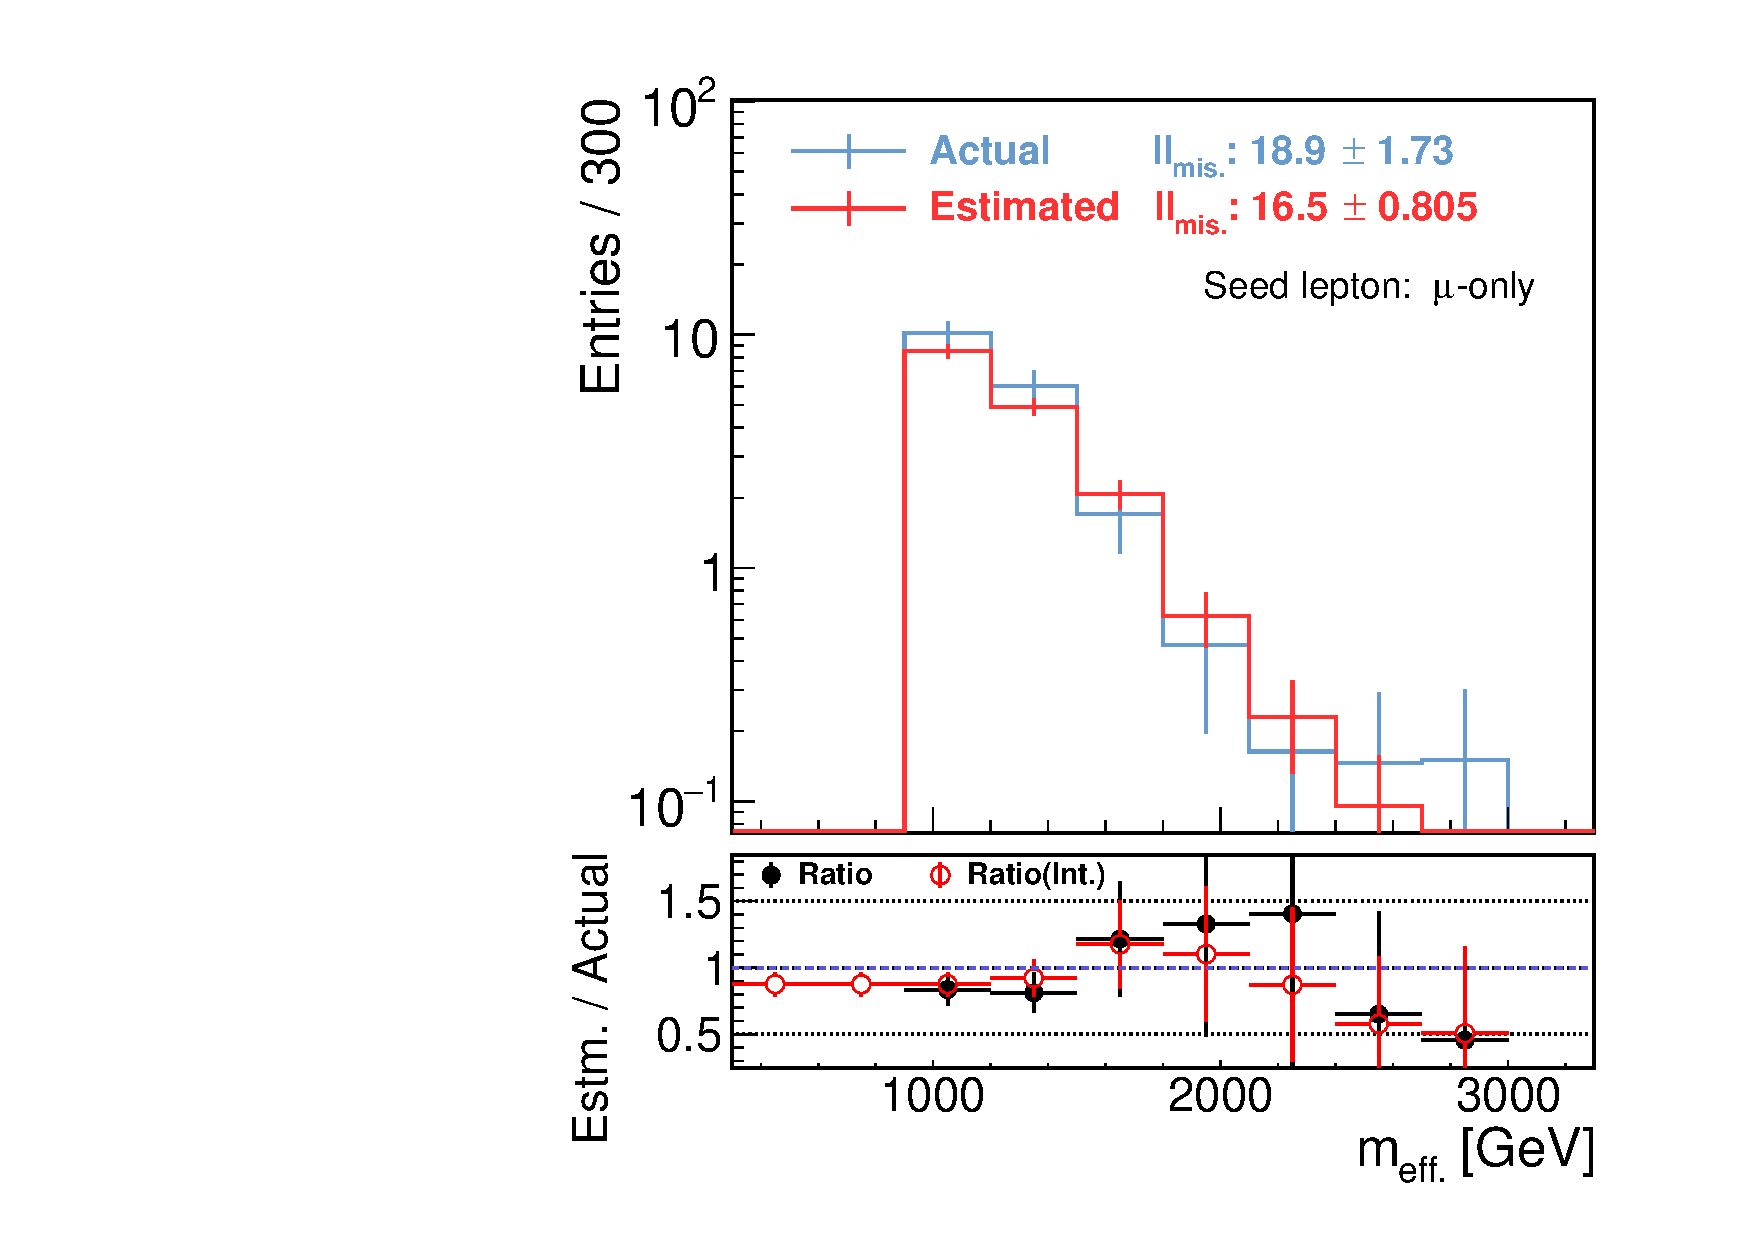
\includegraphics[width=0.32\textwidth]{figures/BGestimation/ObjReplacement/mcClosure_softLep/MisLep_mu_softLep/MisLep_mu_meffInc30__trMode4_NoSys_softLep.pdf}}
    \subfigure[]{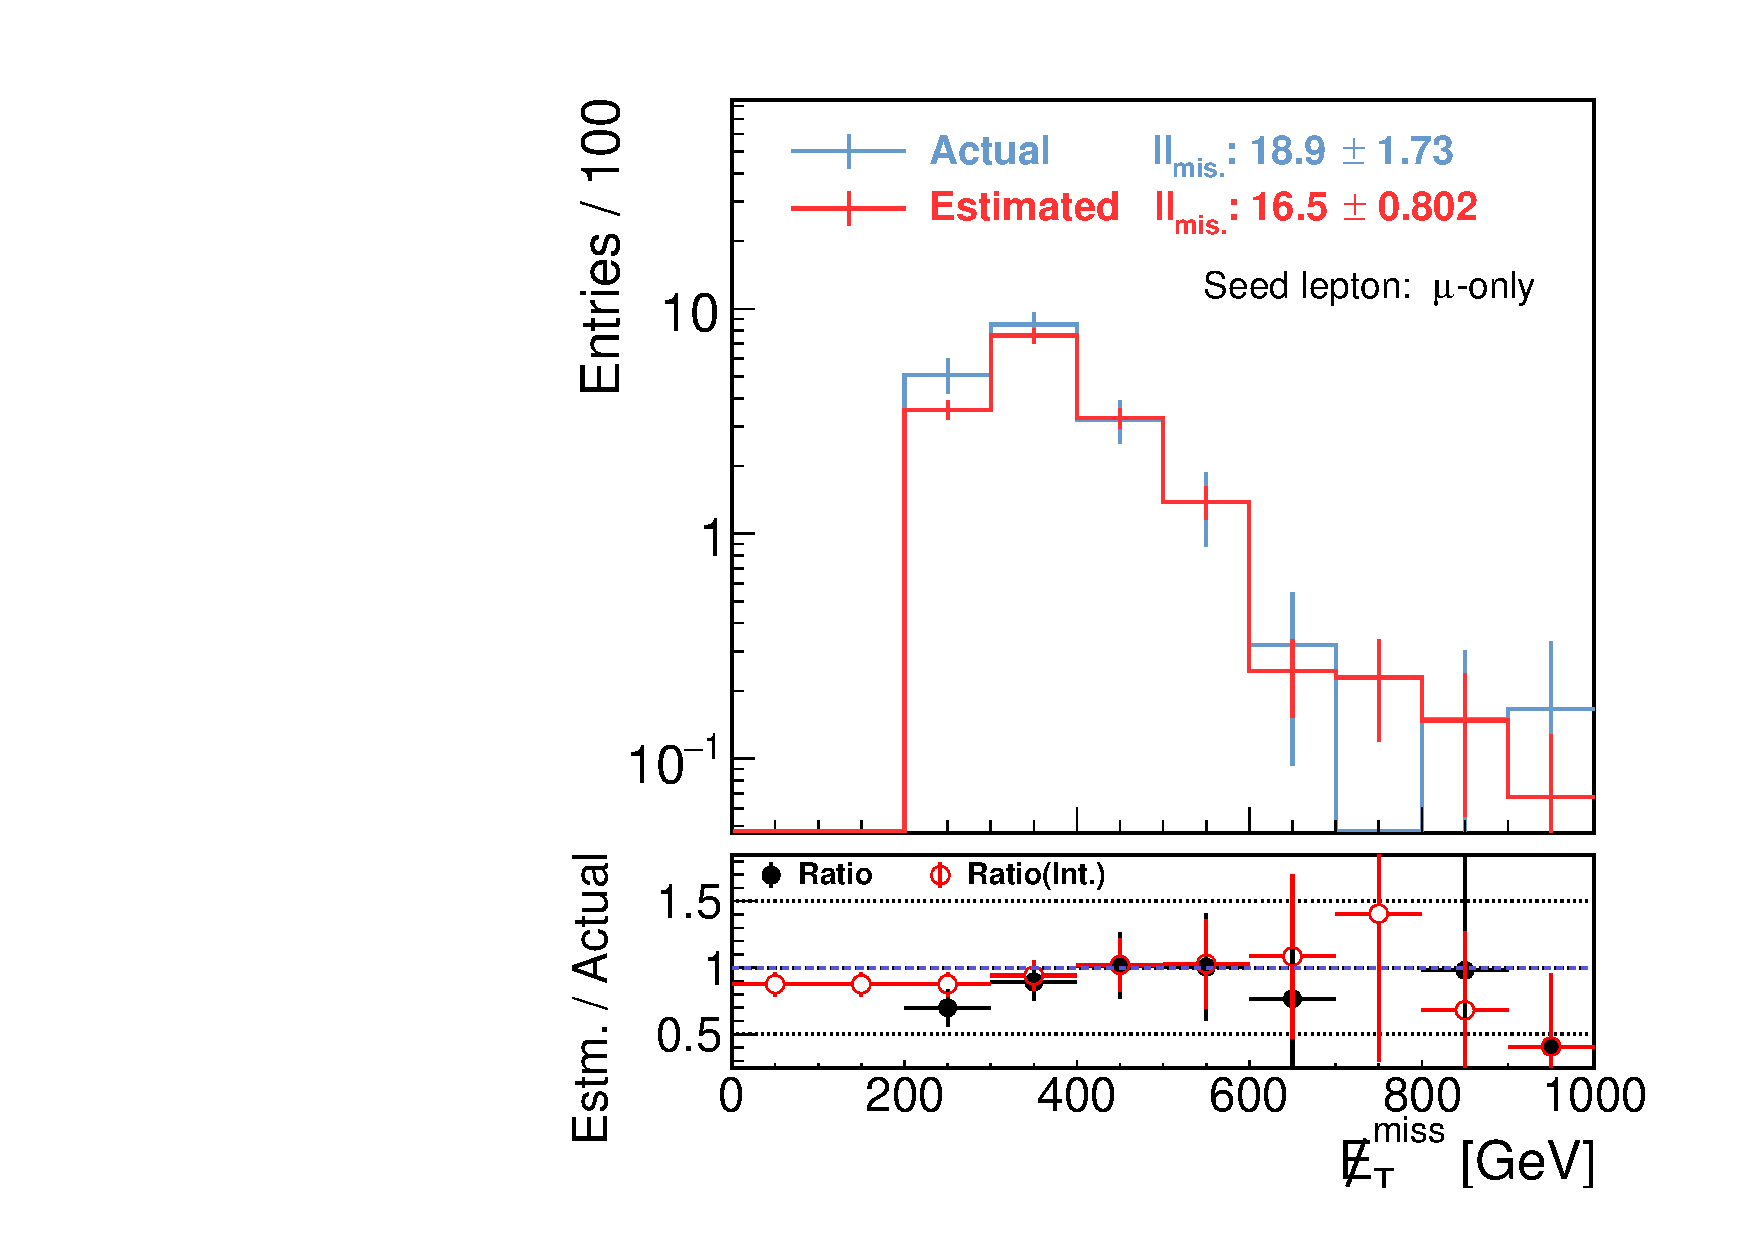
\includegraphics[width=0.32\textwidth]{figures/BGestimation/ObjReplacement/mcClosure_softLep/MisLep_mu_softLep/MisLep_mu_met__trMode4_NoSys_softLep.pdf}}
    \subfigure[]{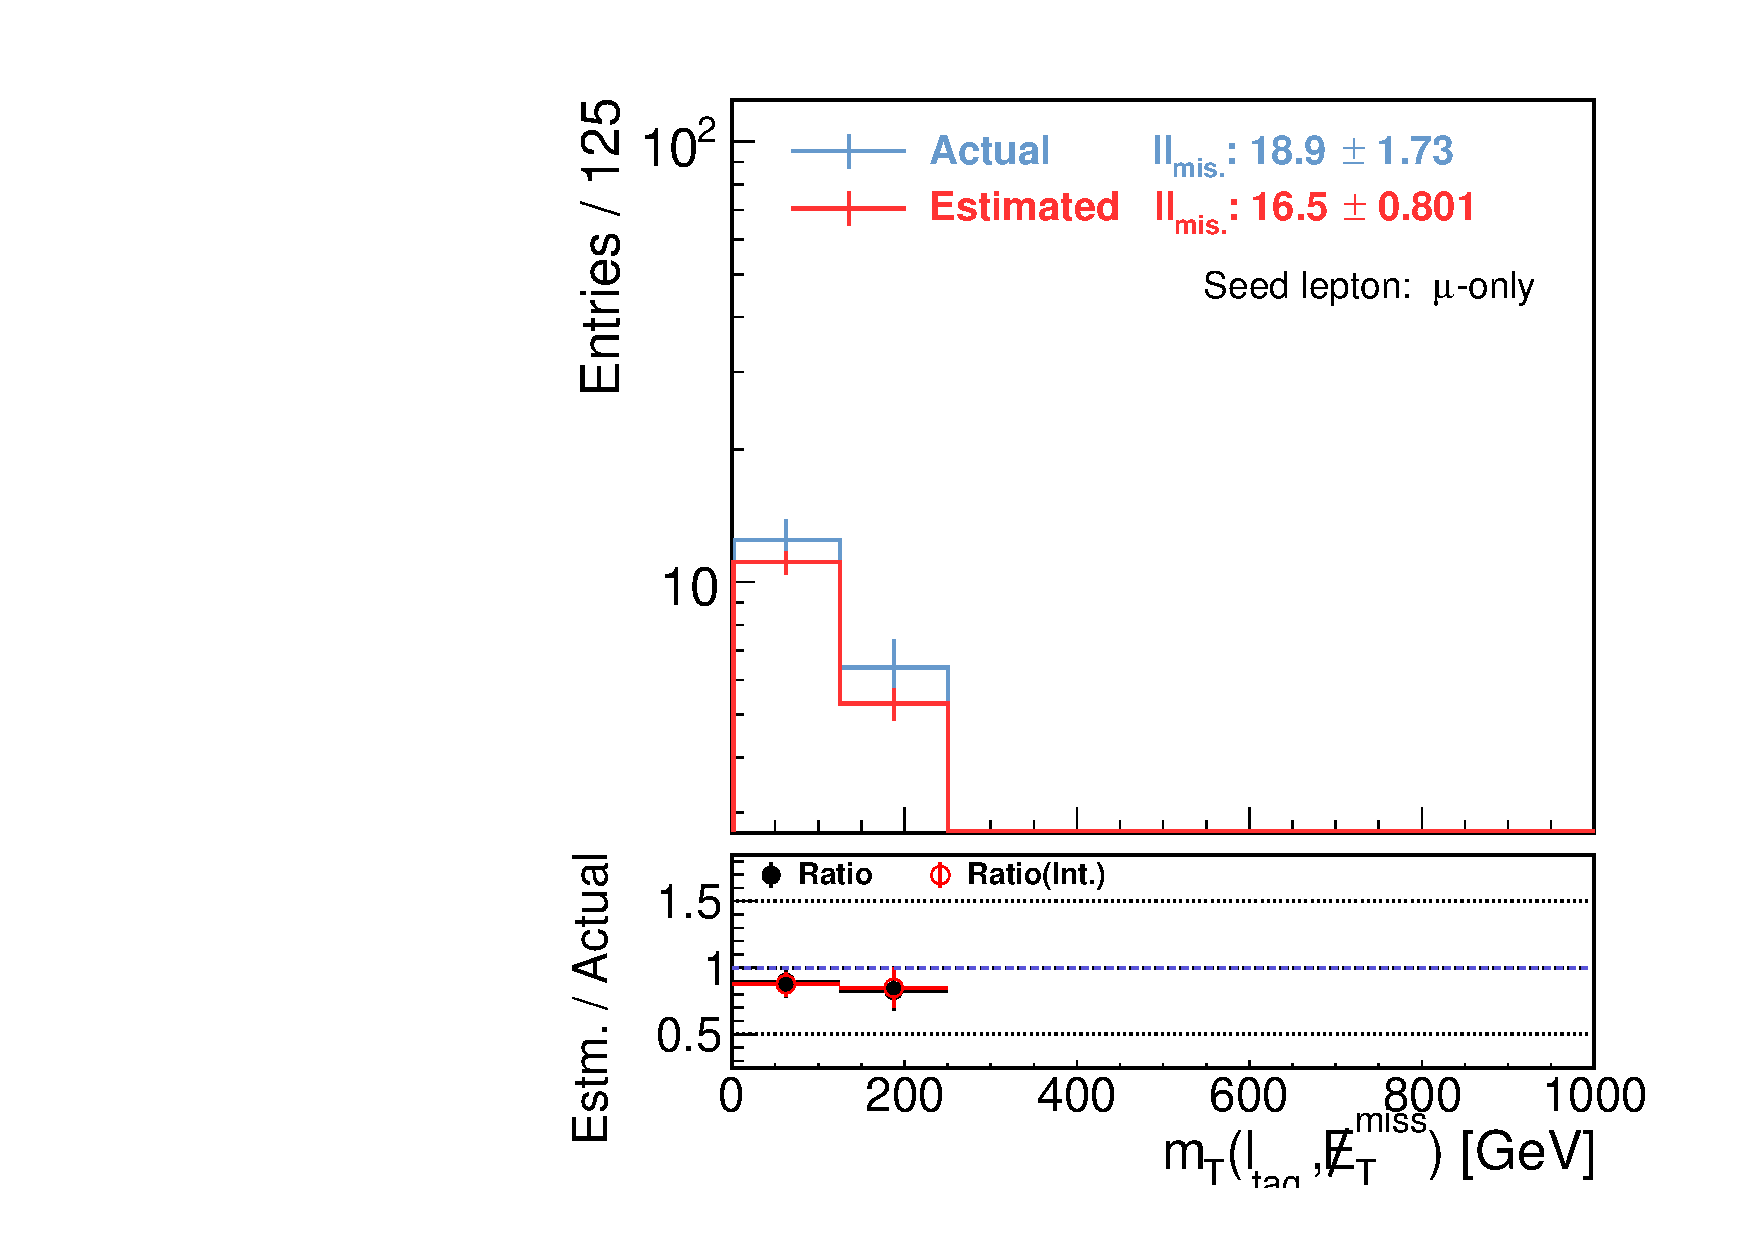
\includegraphics[width=0.32\textwidth]{figures/BGestimation/ObjReplacement/mcClosure_softLep/MisLep_mu_softLep/MisLep_mu_mt__trMode4_NoSys_softLep.pdf}}
    \subfigure[]{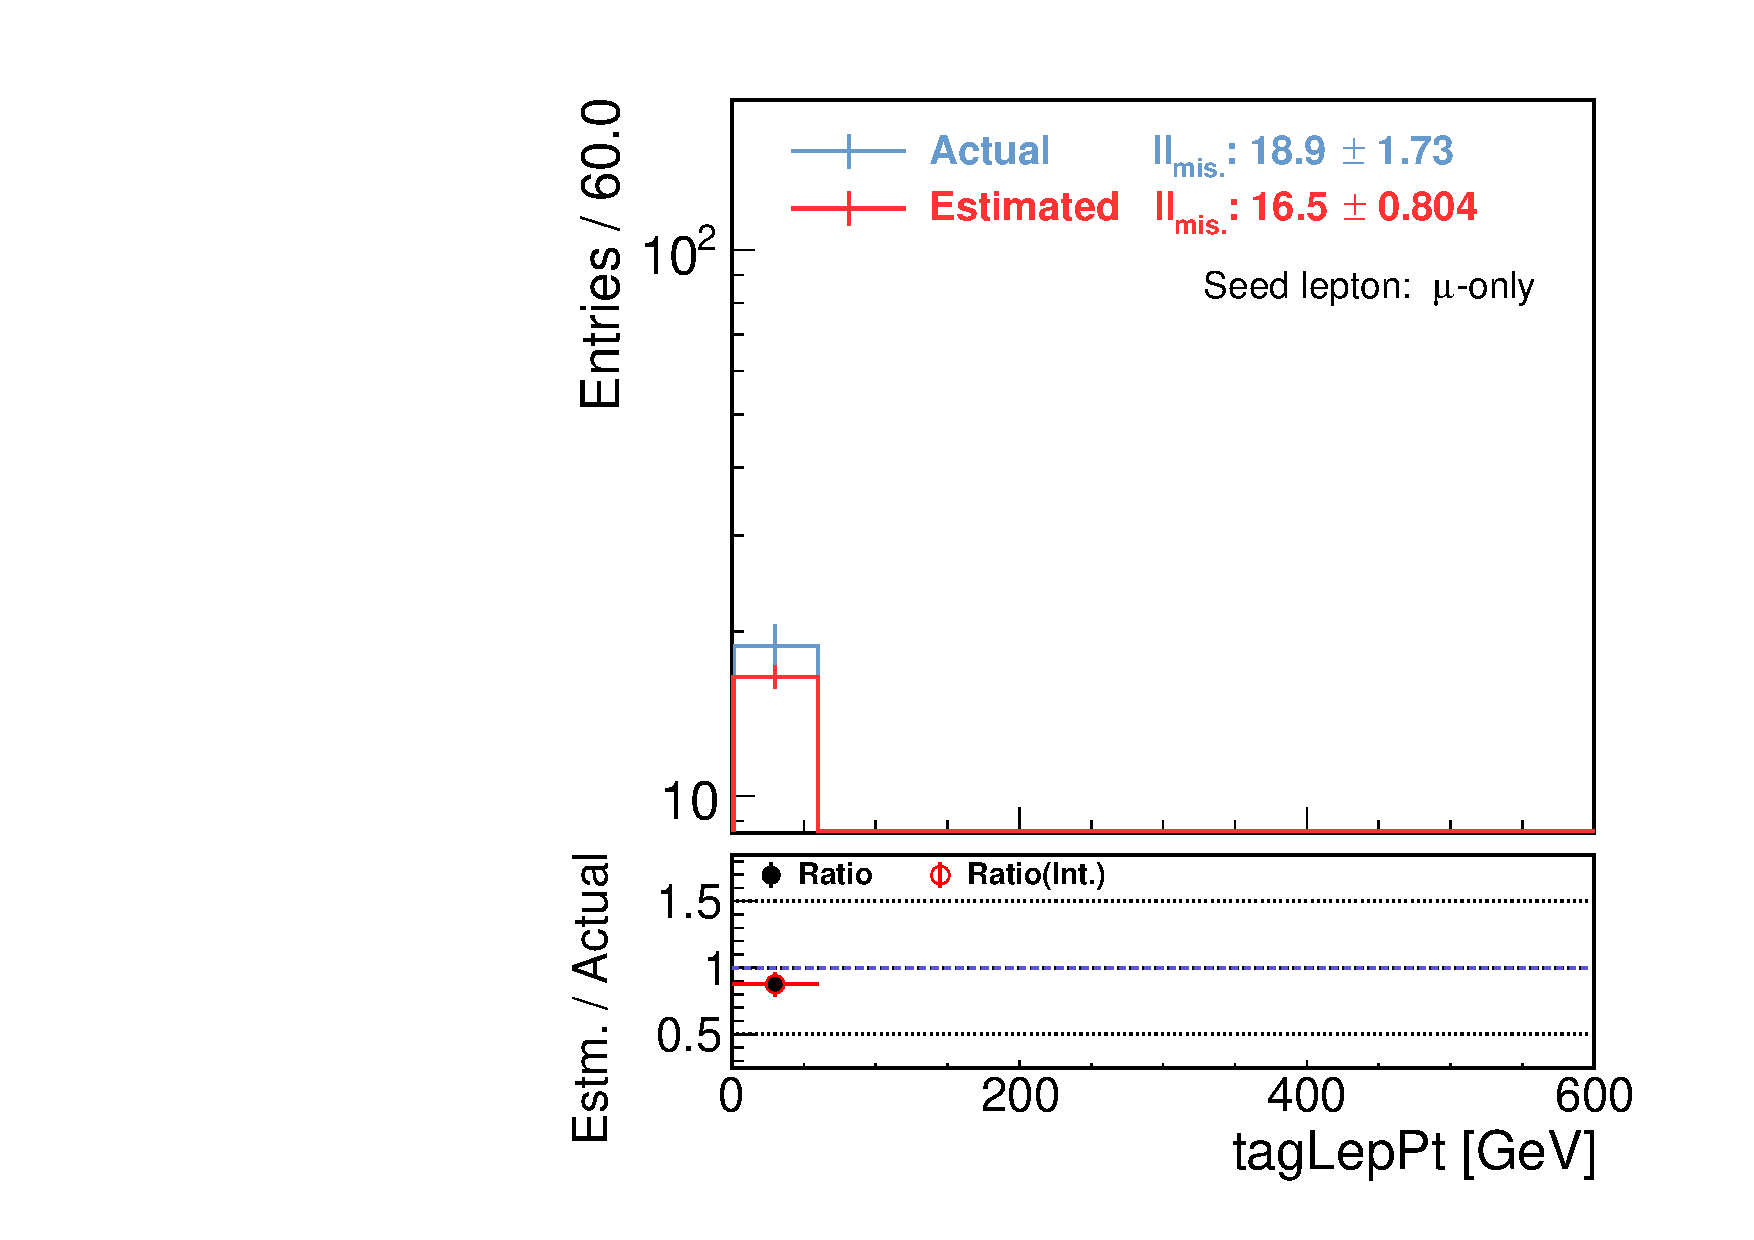
\includegraphics[width=0.32\textwidth]{figures/BGestimation/ObjReplacement/mcClosure_softLep/MisLep_mu_softLep/MisLep_mu_tagLepPt__trMode4_NoSys_softLep.pdf}}
    \subfigure[]{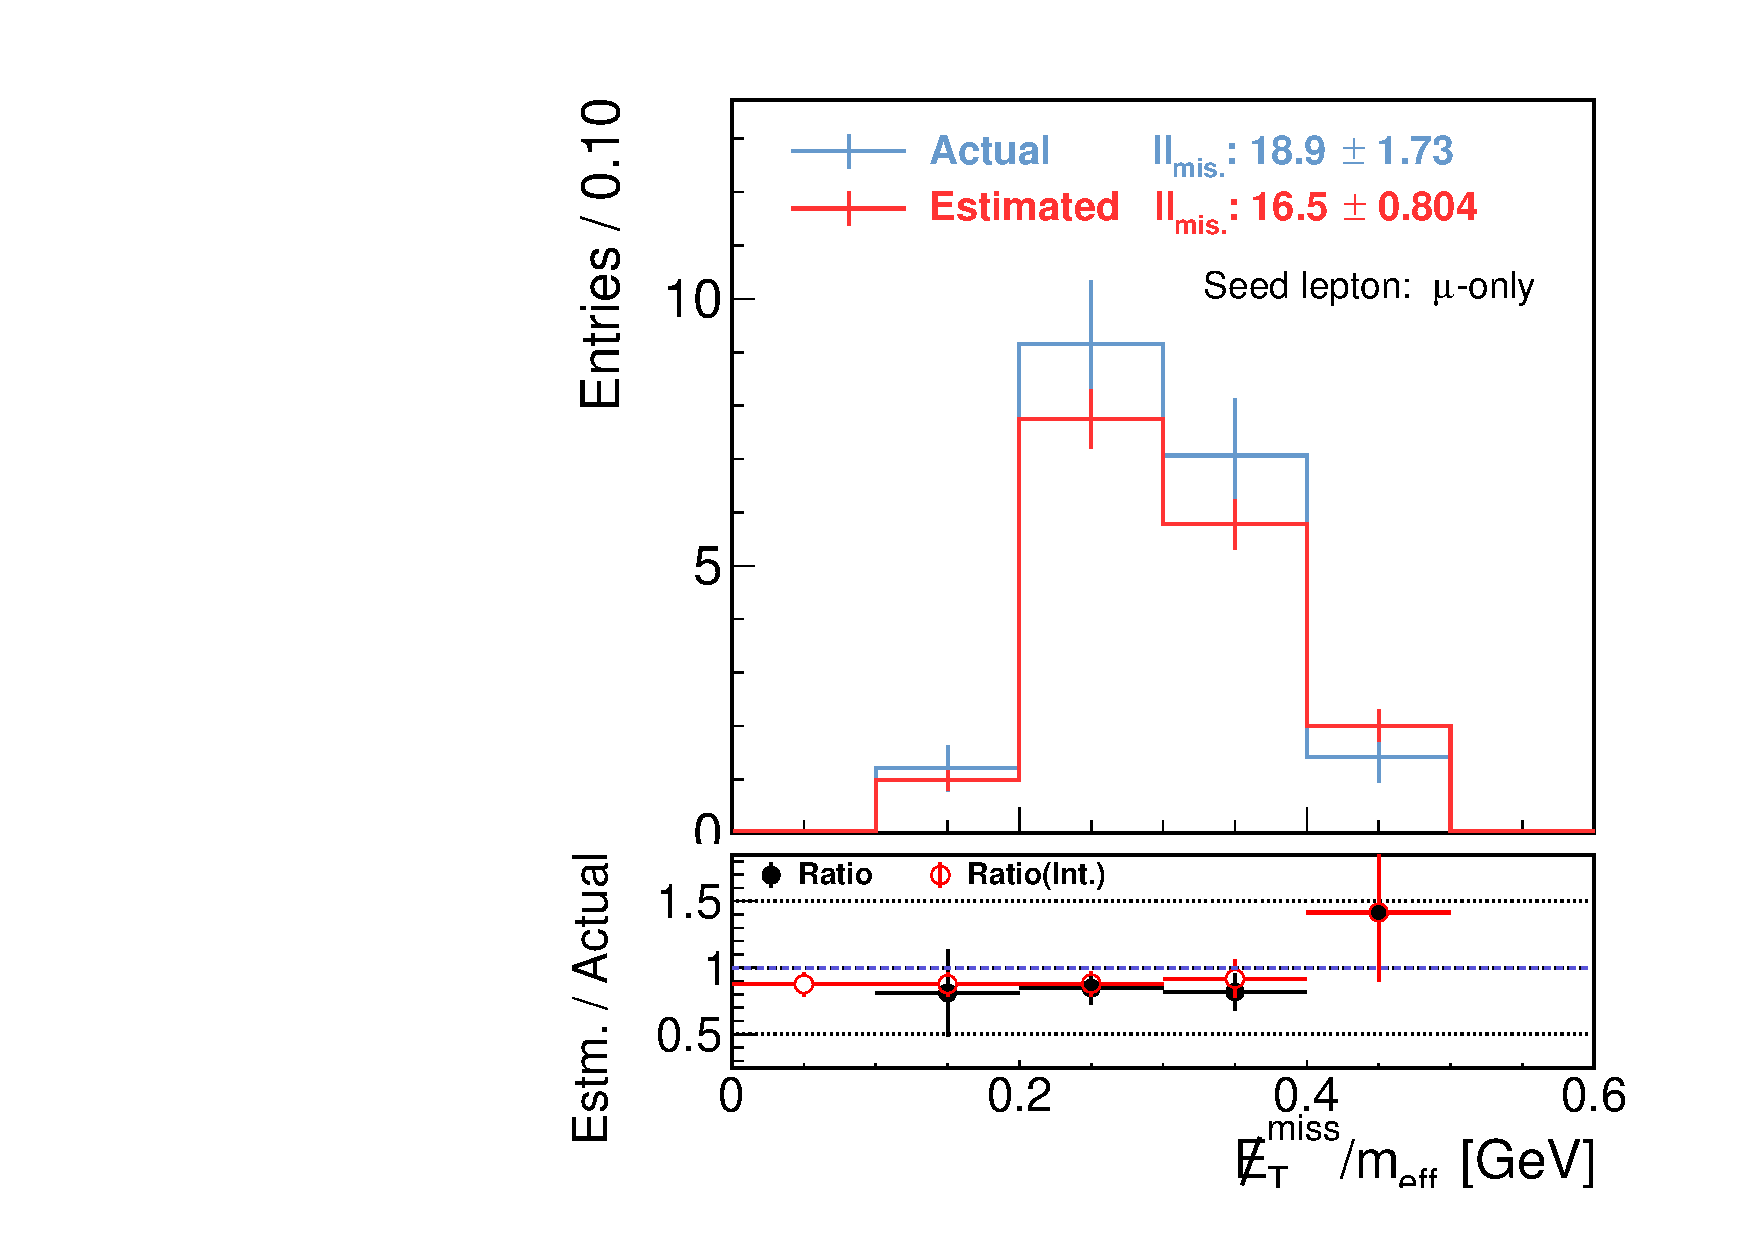
\includegraphics[width=0.32\textwidth]{figures/BGestimation/ObjReplacement/mcClosure_softLep/MisLep_mu_softLep/MisLep_mu_metOverMeff__trMode4_NoSys_softLep.pdf}}
    \subfigure[]{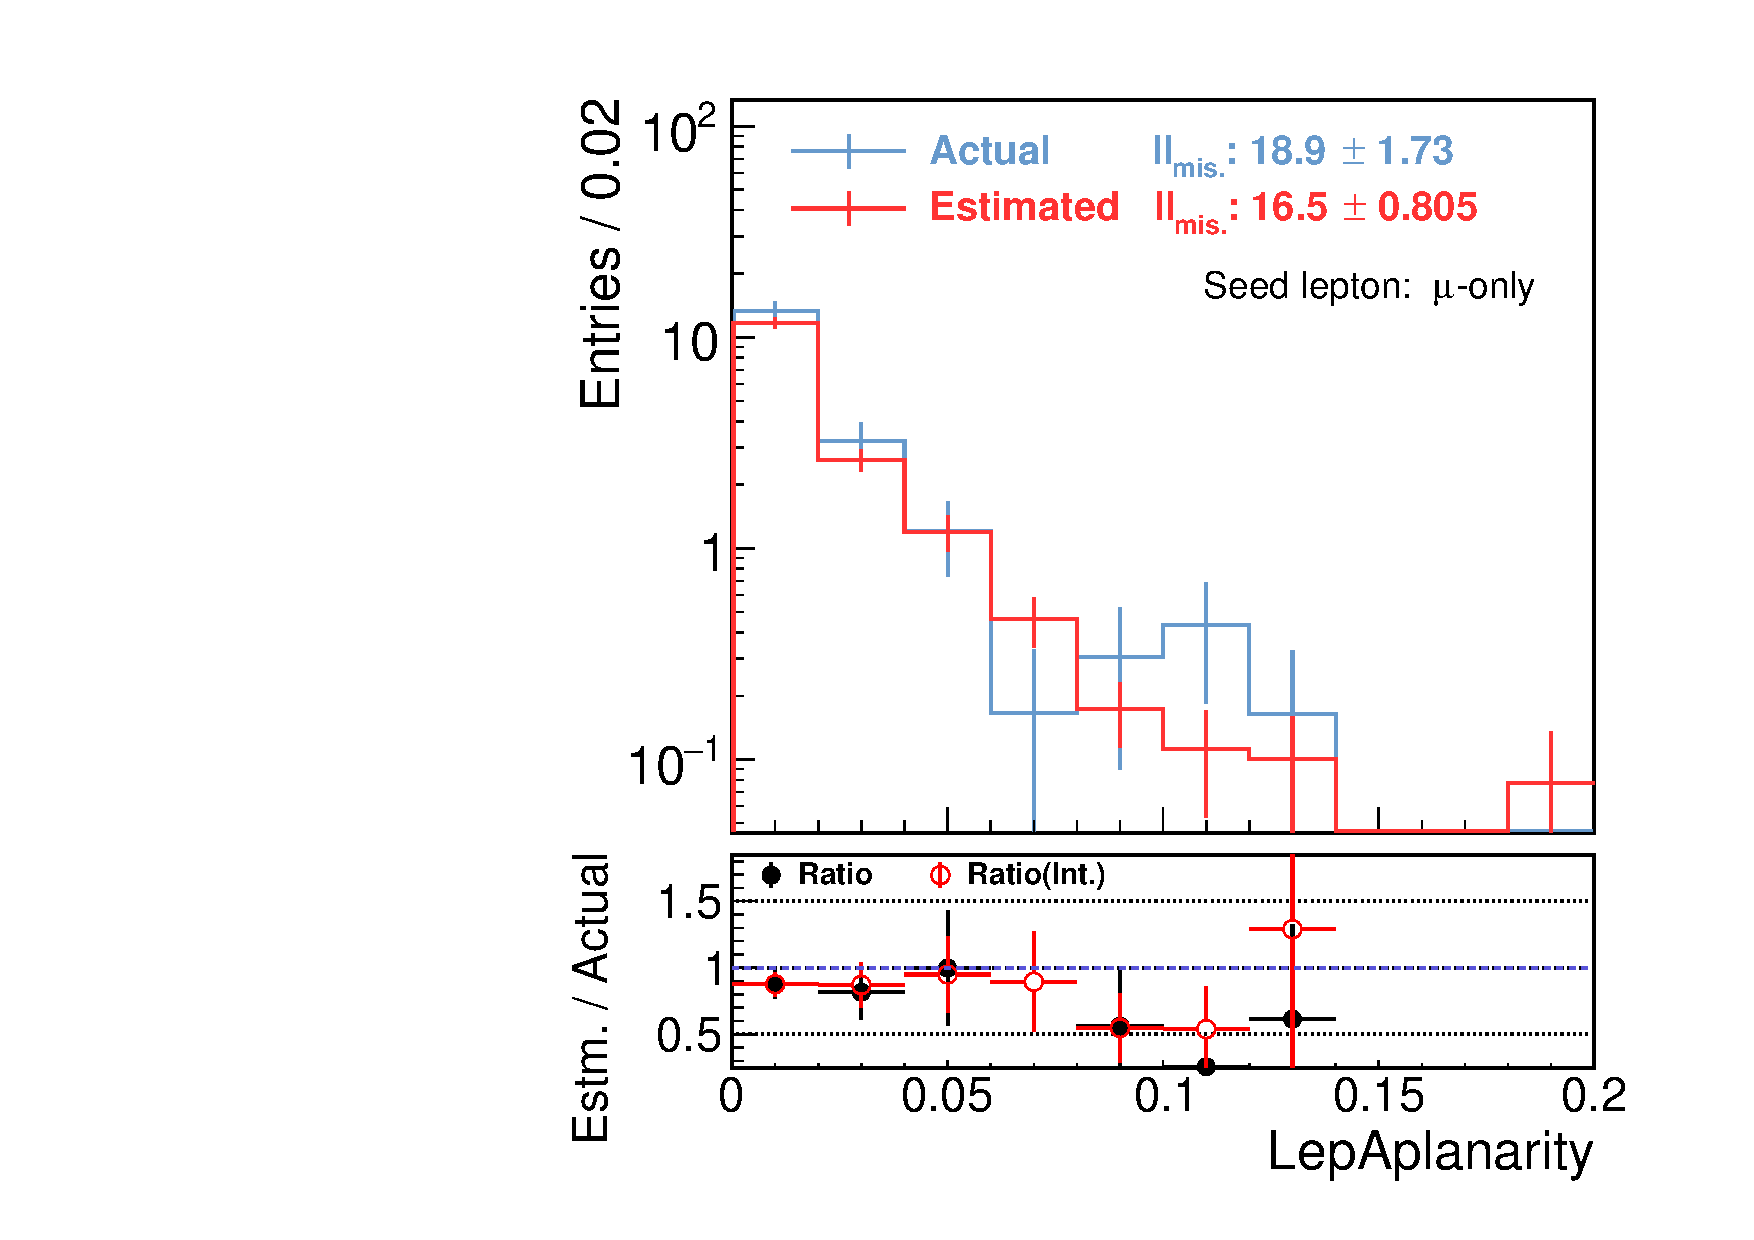
\includegraphics[width=0.32\textwidth]{figures/BGestimation/ObjReplacement/mcClosure_softLep/MisLep_mu_softLep/MisLep_mu_LepAplanarity__trMode4_NoSys_softLep.pdf}}
    \subfigure[]{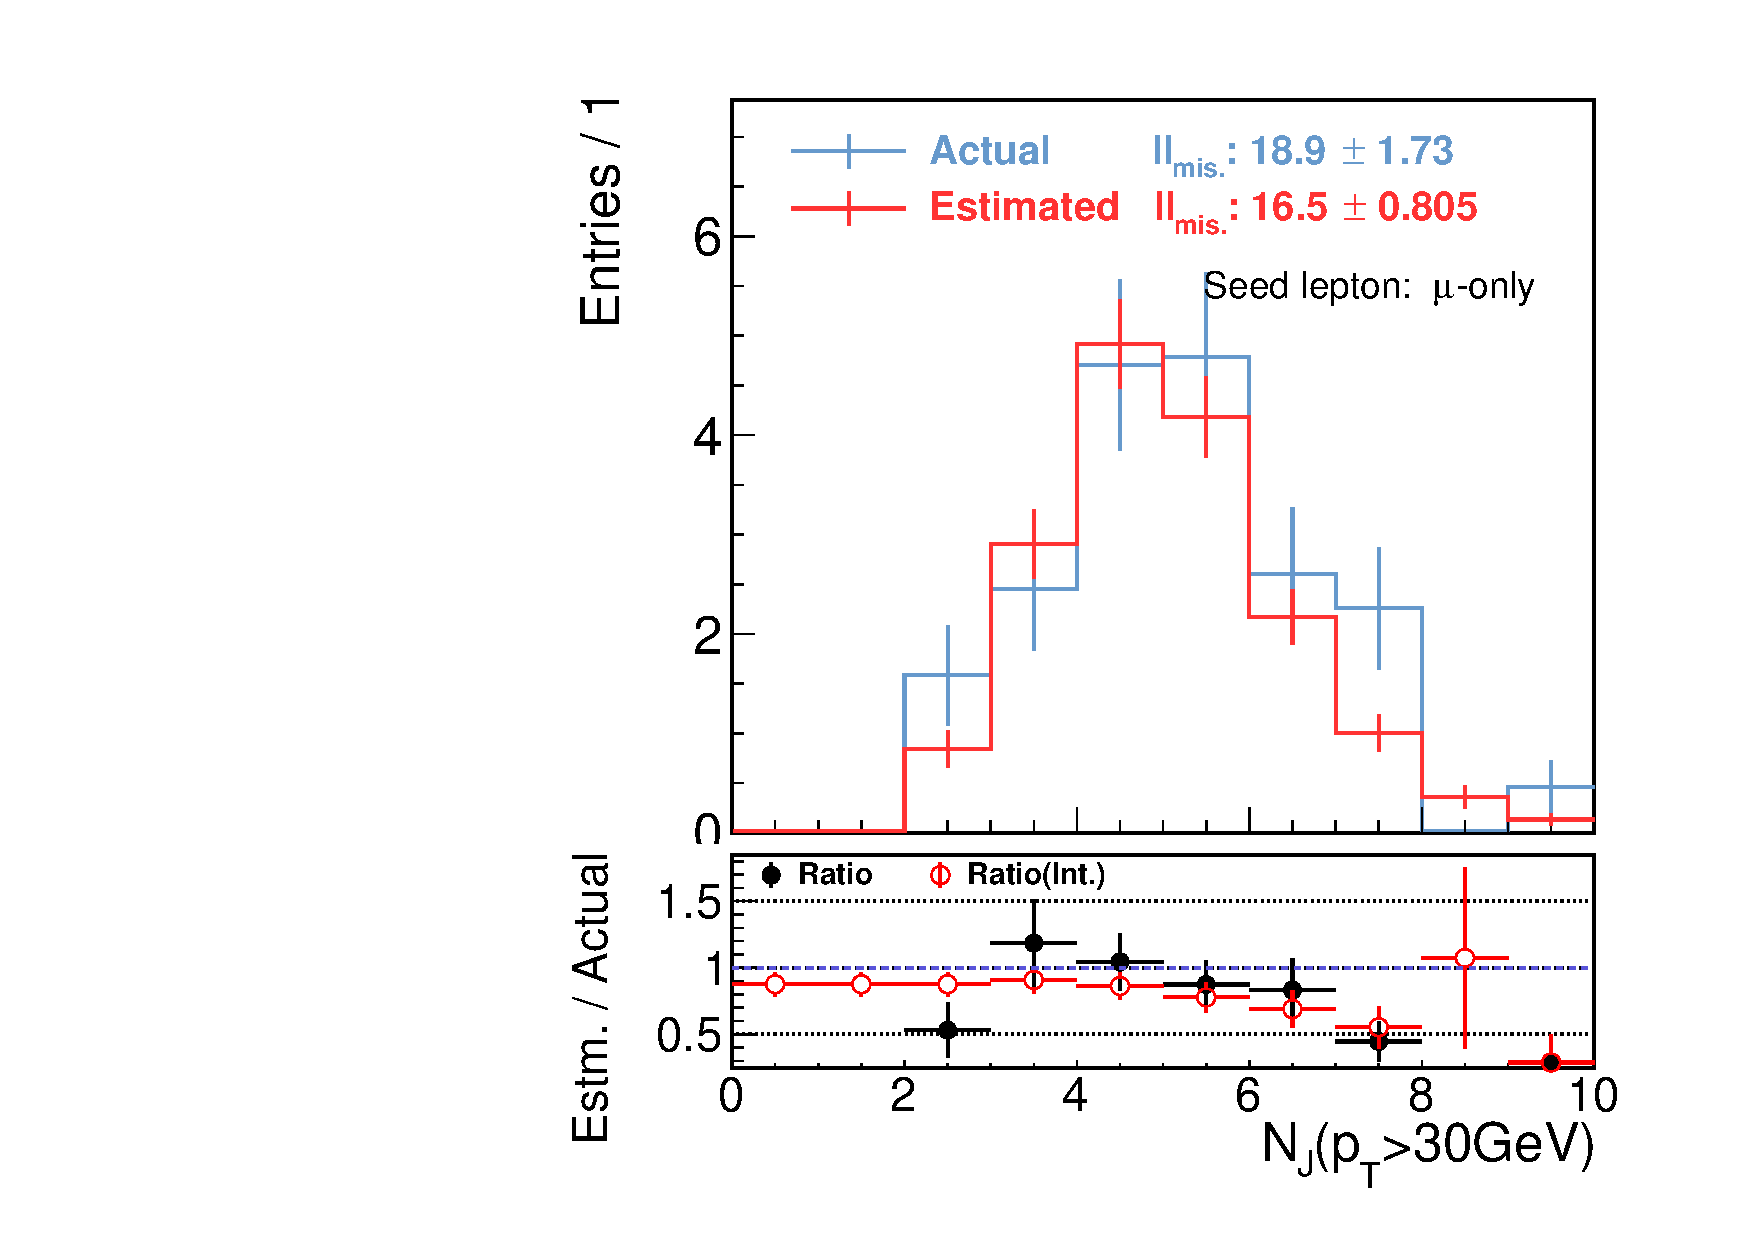
\includegraphics[width=0.32\textwidth]{figures/BGestimation/ObjReplacement/mcClosure_softLep/MisLep_mu_softLep/MisLep_mu_nJet30__trMode4_NoSys_softLep.pdf}}
    \subfigure[]{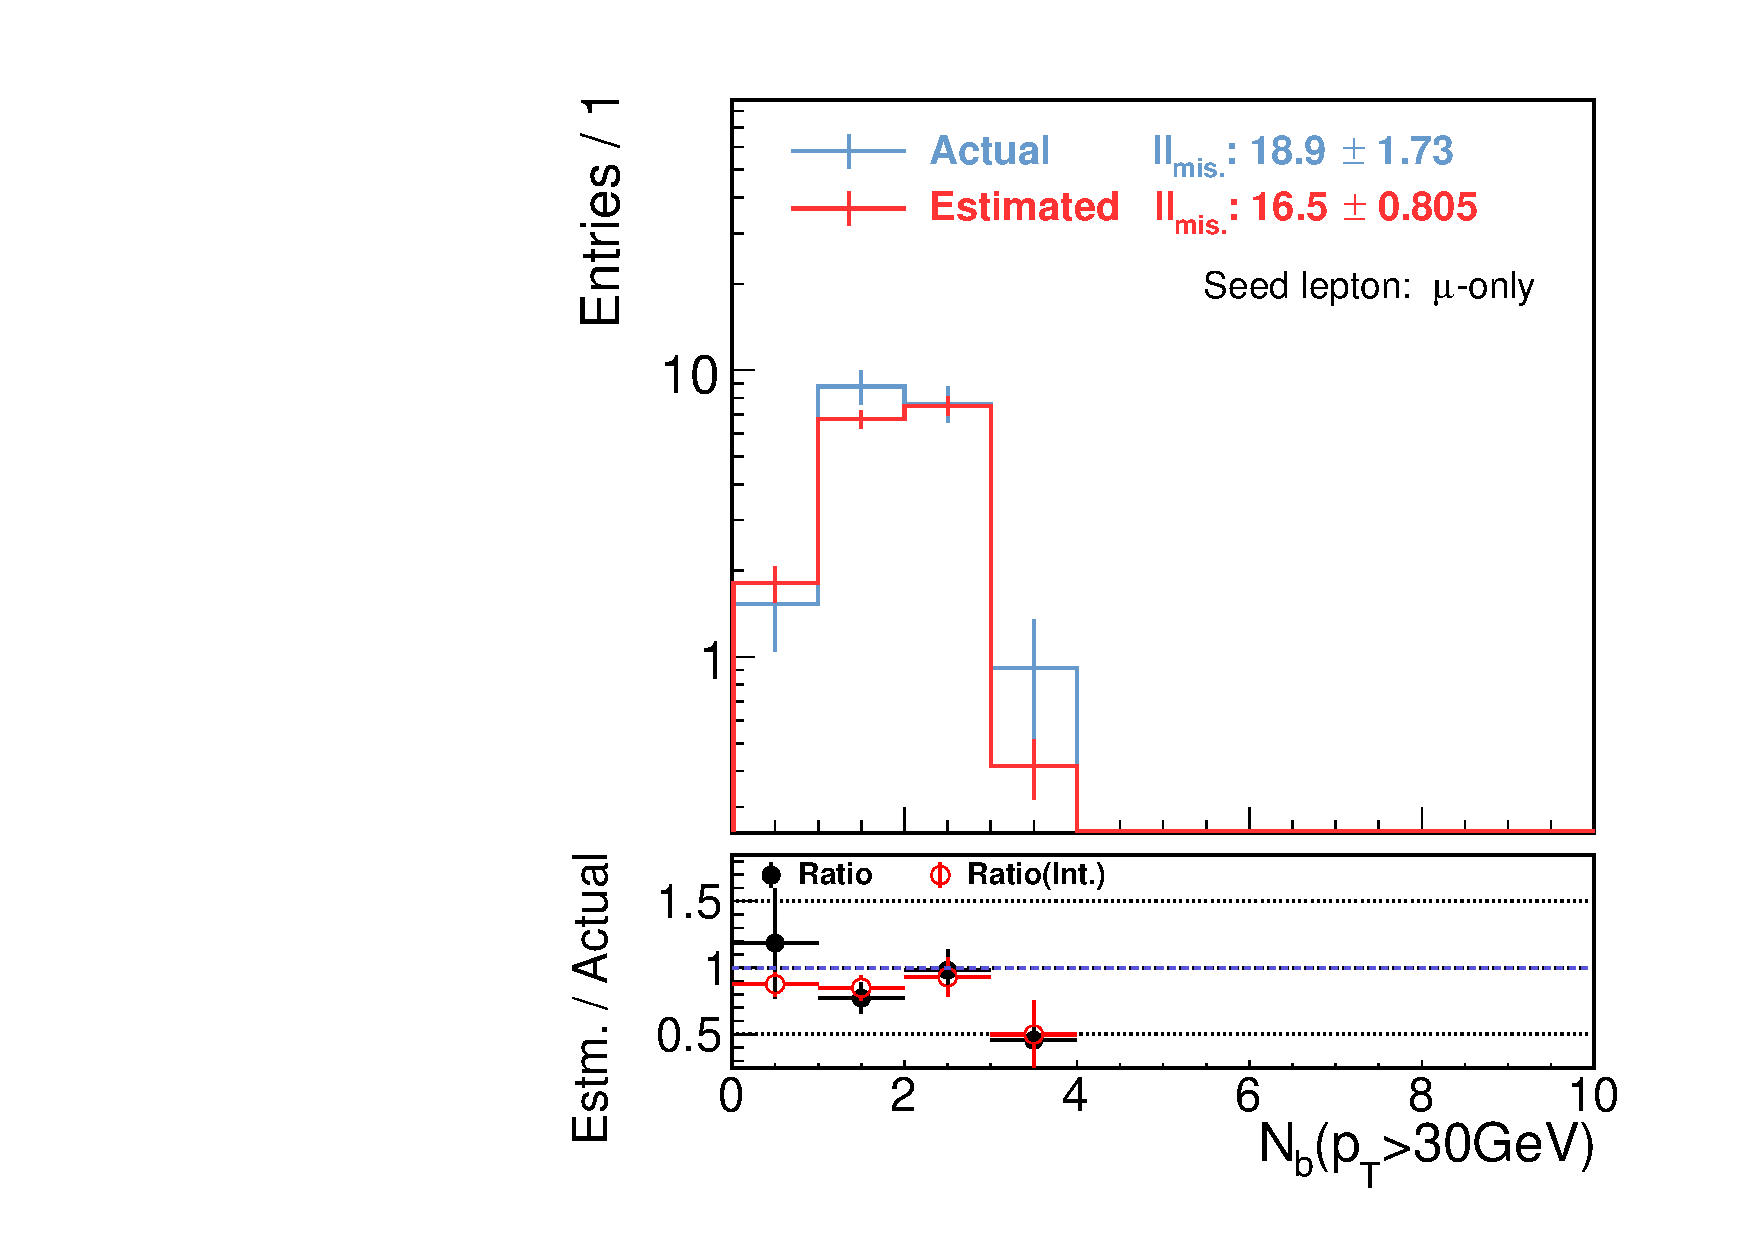
\includegraphics[width=0.32\textwidth]{figures/BGestimation/ObjReplacement/mcClosure_softLep/MisLep_mu_softLep/MisLep_mu_nBJet30__trMode4_NoSys_softLep.pdf}}
    \caption{ MC closure test for \textbf{missing lepton replacement} using $t\bar{t}$ MC sample. Seed events are collected by the use of MET trigger. $p_T<35\gev$ for the leading lepton is required. \textbf{Only muon in the seed events are replaced}. Red points in the bottom plots show the ratio of integrated yields for the two histograms above the x-position that the point indicates. \label{fig::ObjReplace::mcClosure_softLep_MisLep_mu} }
\end{figure}
 %%%%%%%%%%%%%%%%%%%%%%%%%%

%%%%% METHNAME %%%%%%%%%%%%%%%%%%%%%%%%%%
\begin{figure}[h]
  \centering
    \subfig{0.32}{figures/BGestimation/ObjReplacement/mcClosure_softLep/TauRep_emu_softLep/TauRep_emu_jet1Pt__trMode4_NoSys_softLep.pdf}{$\pt$ of leading jet}
    \subfig{0.32}{figures/BGestimation/ObjReplacement/mcClosure_softLep/TauRep_emu_softLep/TauRep_emu_meffInc30__trMode4_NoSys_softLep.pdf}{$\meffInc$}
    \subfig{0.32}{figures/BGestimation/ObjReplacement/mcClosure_softLep/TauRep_emu_softLep/TauRep_emu_met__trMode4_NoSys_softLep.pdf}{$\met$}
    \subfig{0.32}{figures/BGestimation/ObjReplacement/mcClosure_softLep/TauRep_emu_softLep/TauRep_emu_mt__trMode4_NoSys_softLep.pdf}{$\mt$}
    \subfig{0.32}{figures/BGestimation/ObjReplacement/mcClosure_softLep/TauRep_emu_softLep/TauRep_emu_metOverMeff__trMode4_NoSys_softLep.pdf}{$\met/\meffInc$}
    \subfig{0.32}{figures/BGestimation/ObjReplacement/mcClosure_softLep/TauRep_emu_softLep/TauRep_emu_LepAplanarity__trMode4_NoSys_softLep.pdf}{Aplanarity}
    \subfig{0.32}{figures/BGestimation/ObjReplacement/mcClosure_softlep/TauRep_emu_softLep/TauRep_emu_min_dPhi_4j__trMode4_NoSys_softLep.pdf}{$\mindPhiFourJet$}
    \subfig{0.32}{figures/BGestimation/ObjReplacement/mcClosure_softLep/TauRep_emu_softLep/TauRep_emu_nJet30__trMode4_NoSys_softLep.pdf}{Jet multiplicity}
    \subfig{0.32}{figures/BGestimation/ObjReplacement/mcClosure_softLep/TauRep_emu_softLep/TauRep_emu_nBJet30__trMode4_NoSys_softLep.pdf}{$b$-jet multiplicity}
    \caption{ MC closure test for \textbf{tau replacement} using $t\bar{t}$ MC sample. Seed events are collected by the use of MET trigger. $p_T<35\gev$ for the leading lepton is required. \textbf{Both electrons and muons in the seed events are replaced}. Red points in the bottom plots show the ratio of integrated yields for the two histograms above the x-position that the point indicates. \label{fig::ObjReplace::mcClosure_softLep_TauRep_emu} }
\end{figure}
 %%%%%%%%%%%%%%%%%%%%%%%%%%




%\clearpage
%\paragraph{Combined Test of Missing Lepton Replacement and Tau Replacement} \mbox{} \\
%%%%%% METHNAME %%%%%%%%%%%%%%%%%%%%%%%%%%
\begin{figure}[h]
  \centering
    \subfigure[]{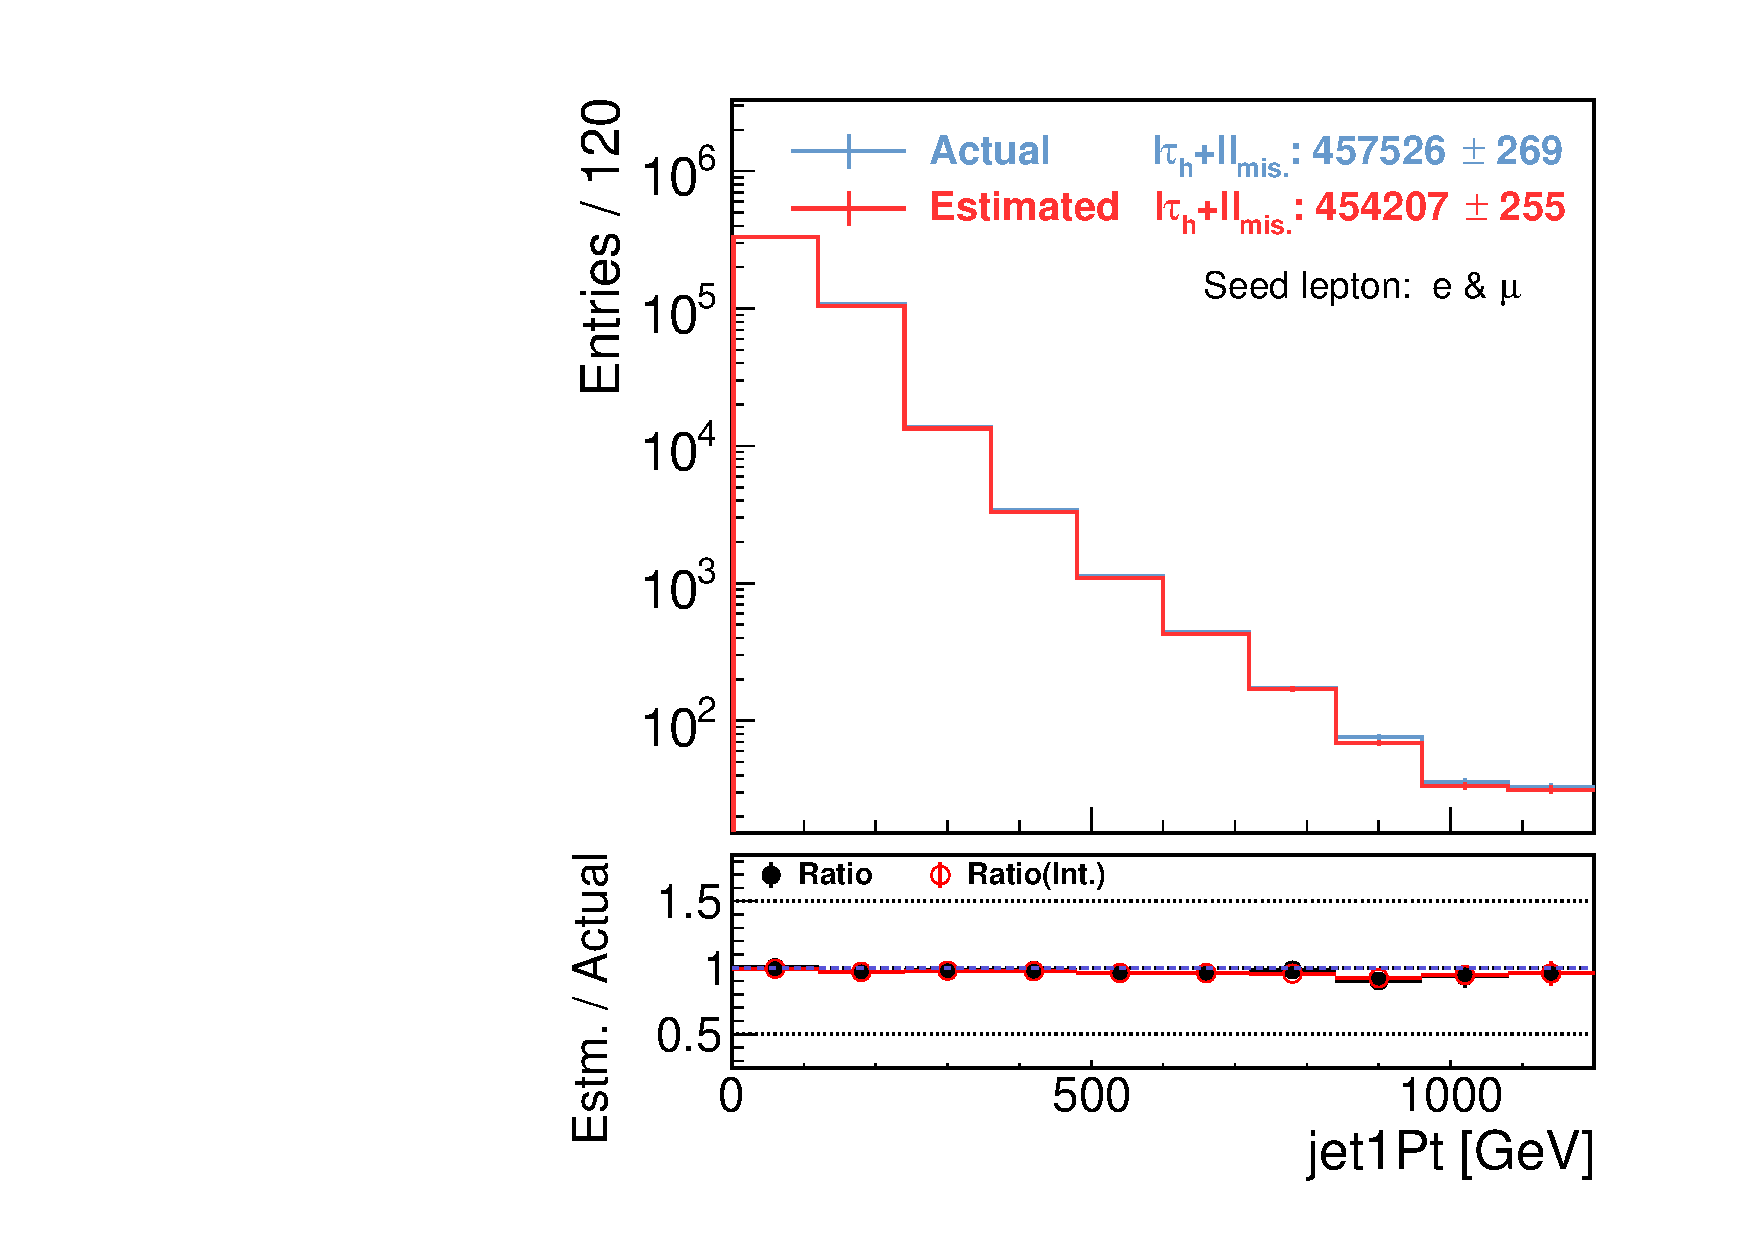
\includegraphics[width=0.32\textwidth]{figures/BGestimation/ObjReplacement/mcClosure/All_emu/All_emu_jet1Pt__trMode4_NoSys.pdf}}
    \subfigure[]{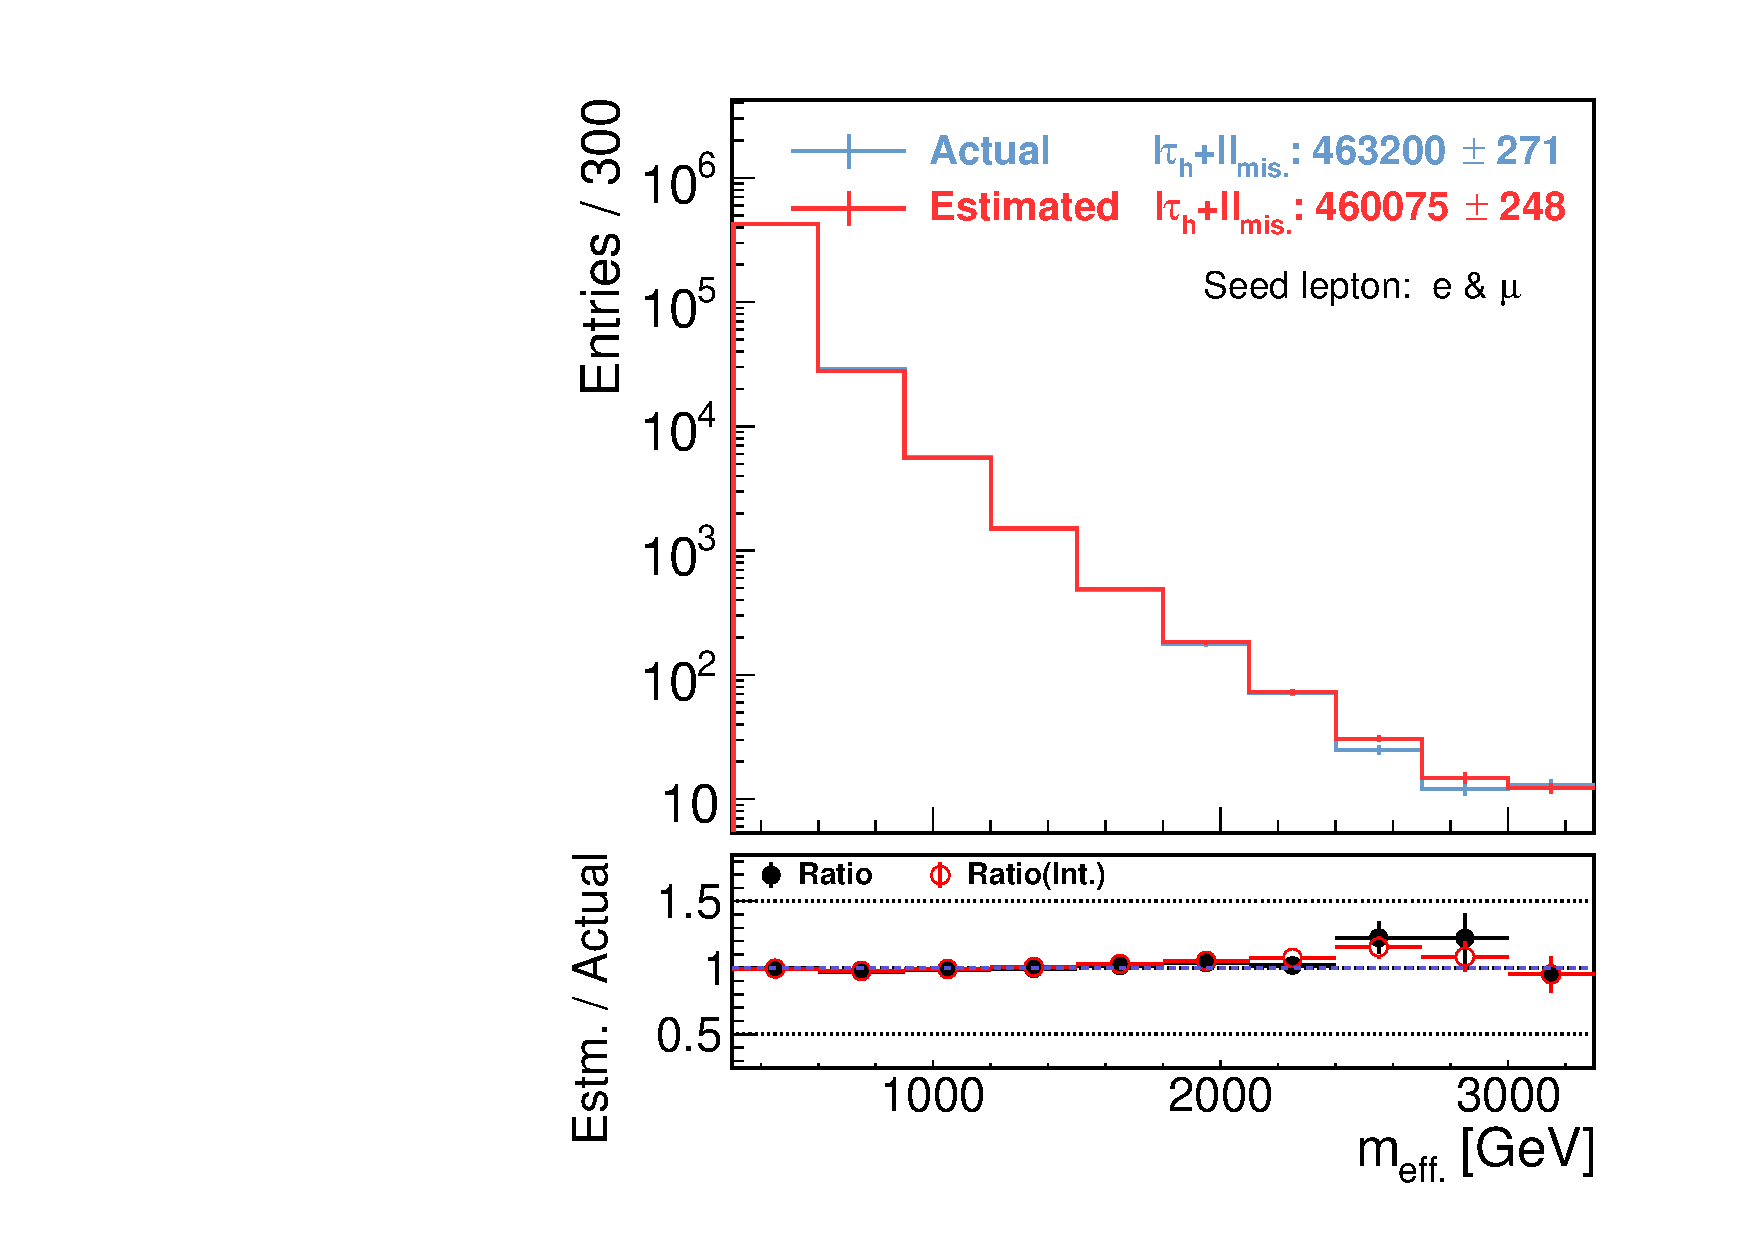
\includegraphics[width=0.32\textwidth]{figures/BGestimation/ObjReplacement/mcClosure/All_emu/All_emu_meffInc30__trMode4_NoSys.pdf}}
    \subfigure[]{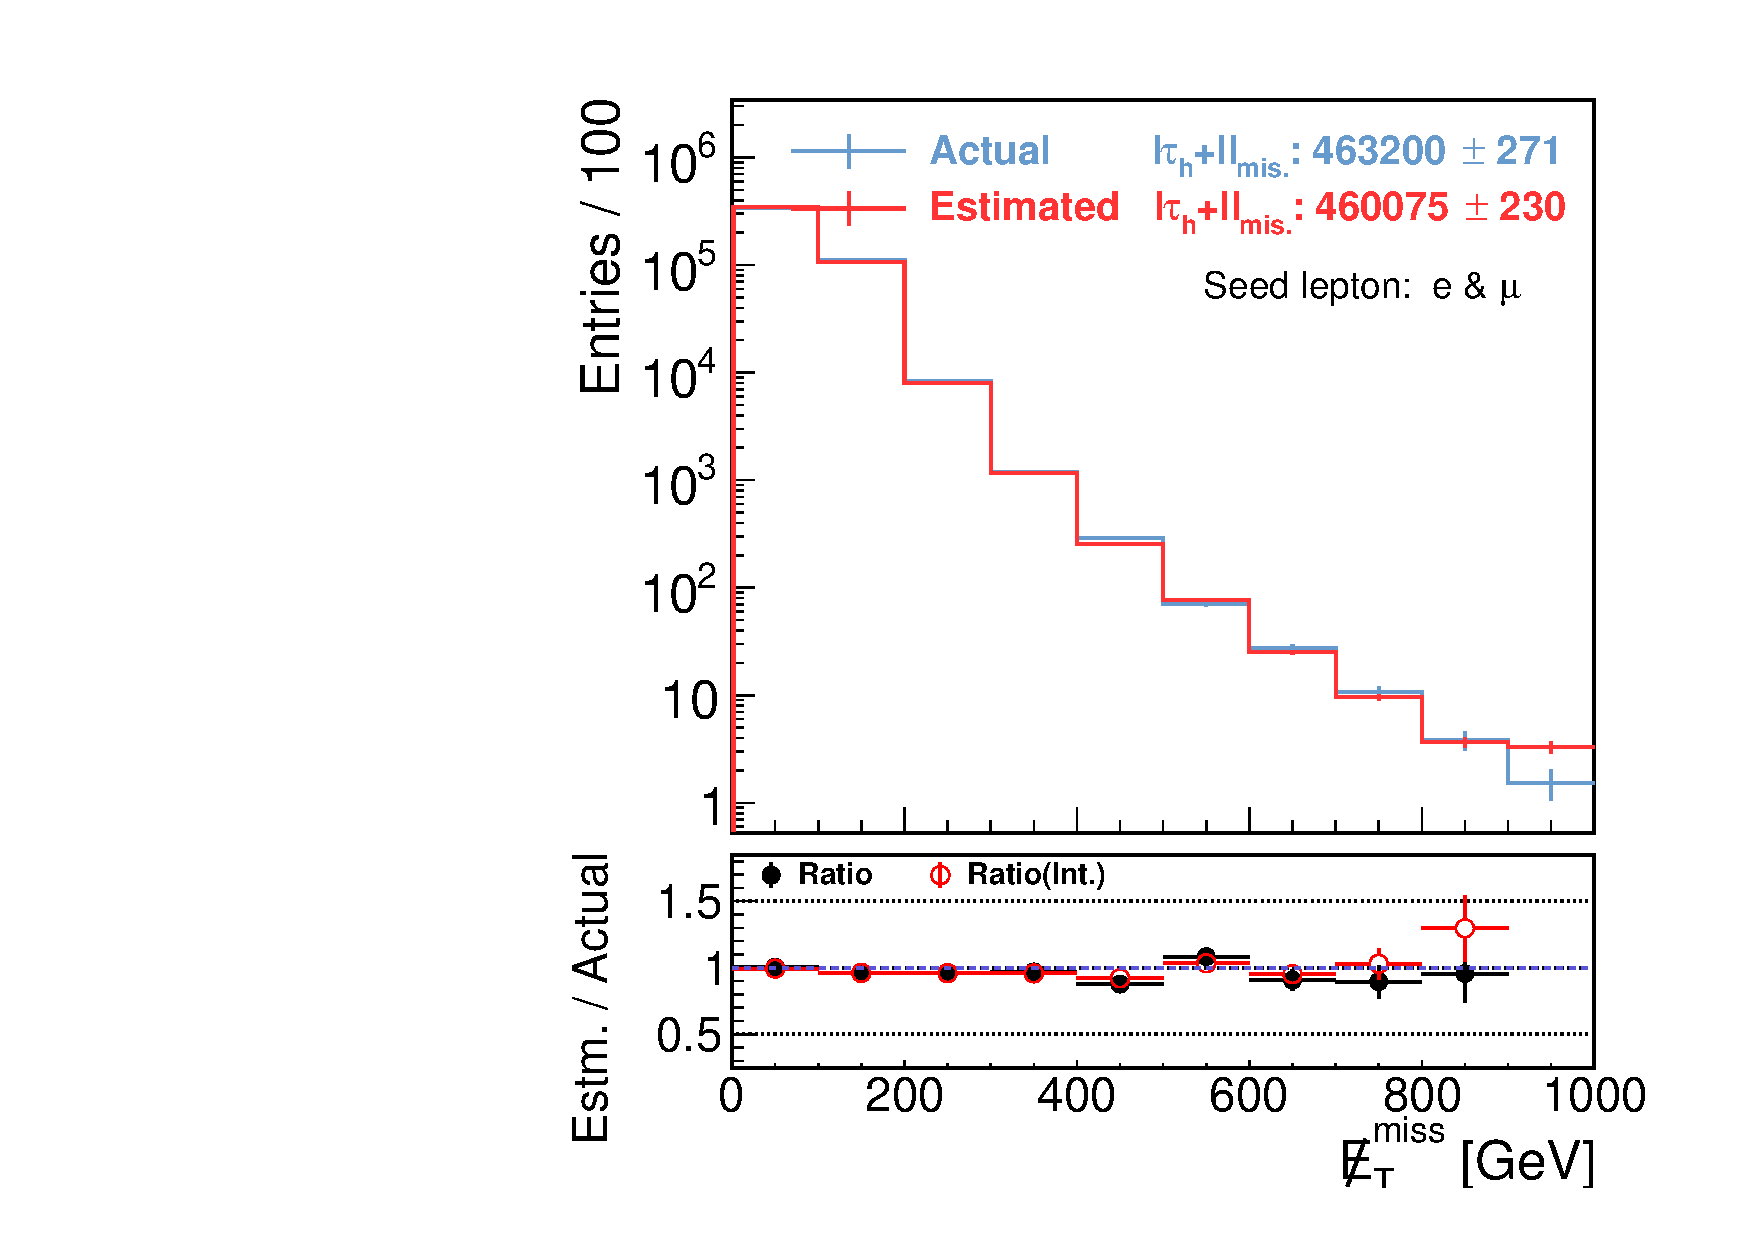
\includegraphics[width=0.32\textwidth]{figures/BGestimation/ObjReplacement/mcClosure/All_emu/All_emu_met__trMode4_NoSys.pdf}}
    \subfigure[]{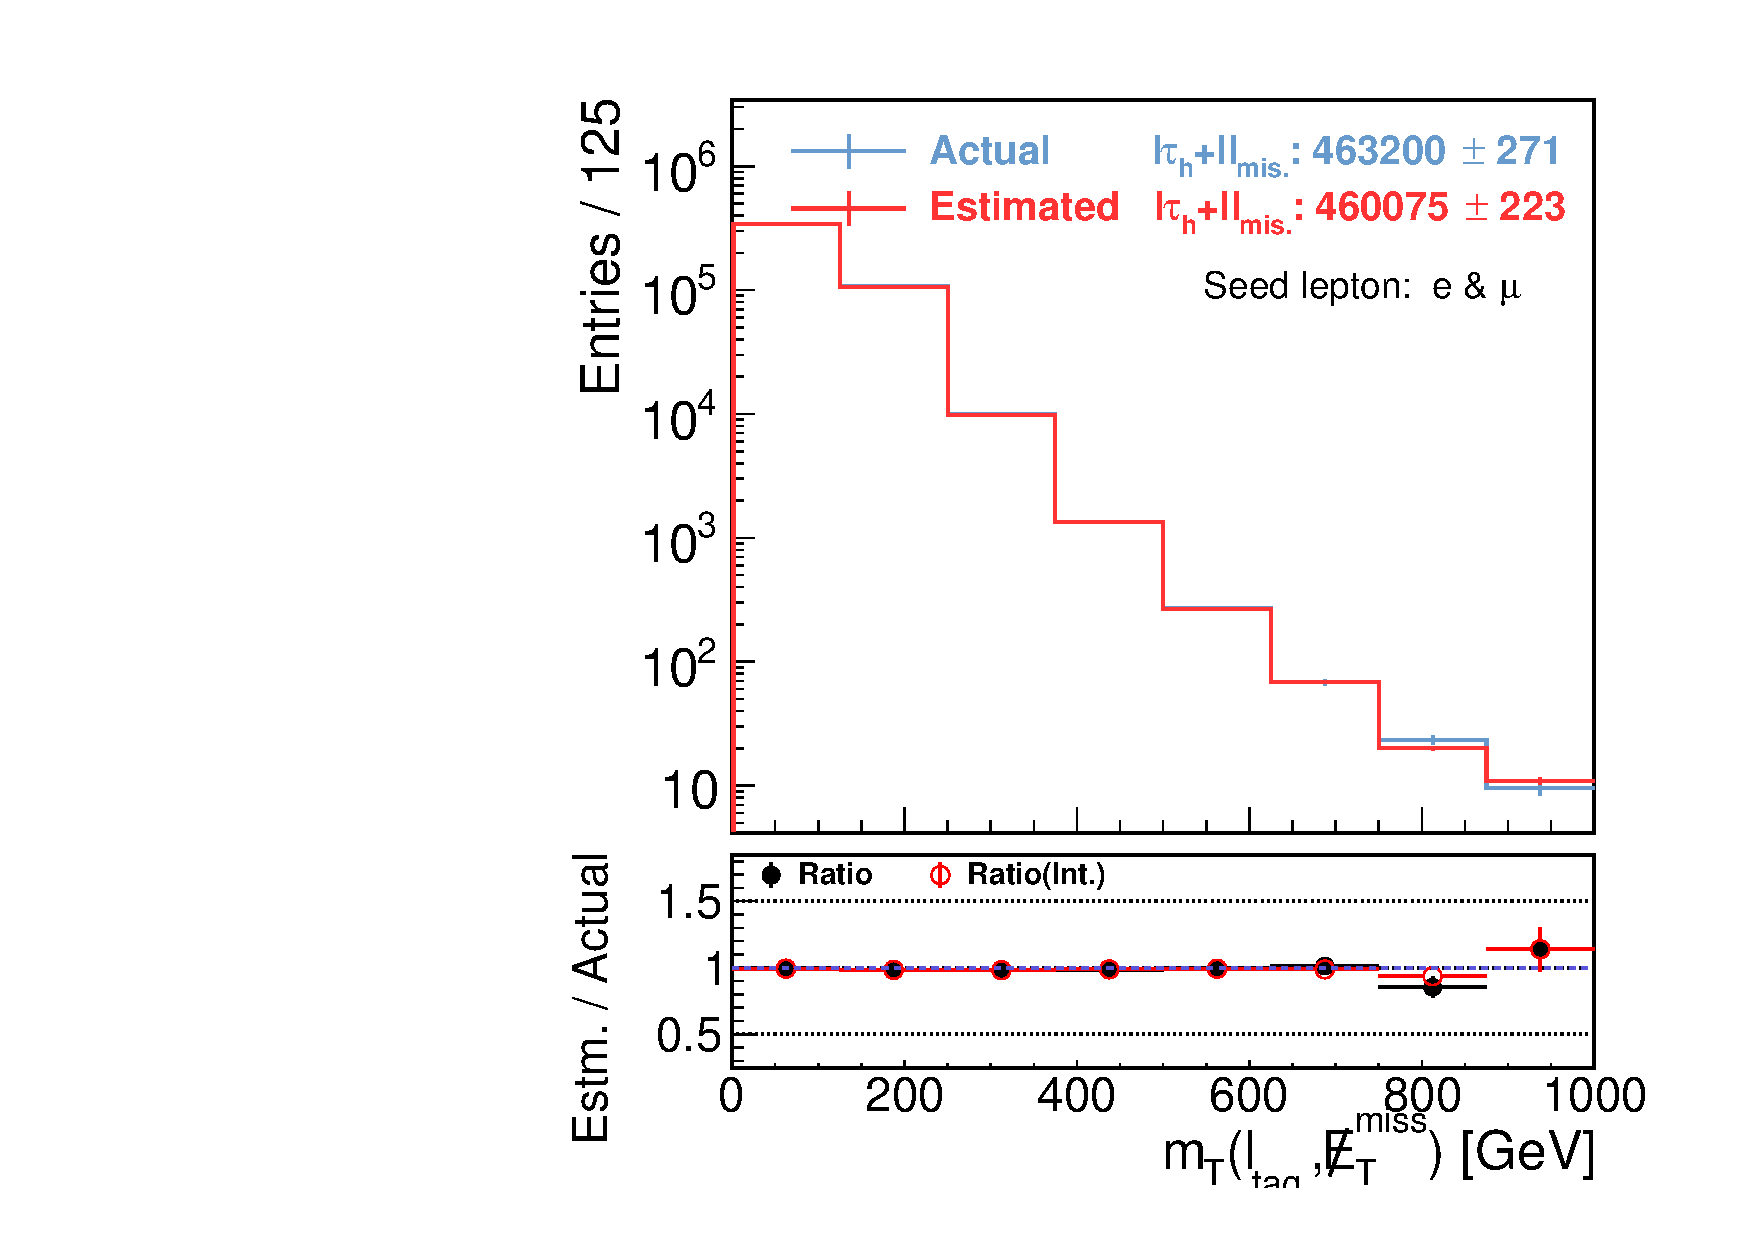
\includegraphics[width=0.32\textwidth]{figures/BGestimation/ObjReplacement/mcClosure/All_emu/All_emu_mt__trMode4_NoSys.pdf}}
    \subfigure[]{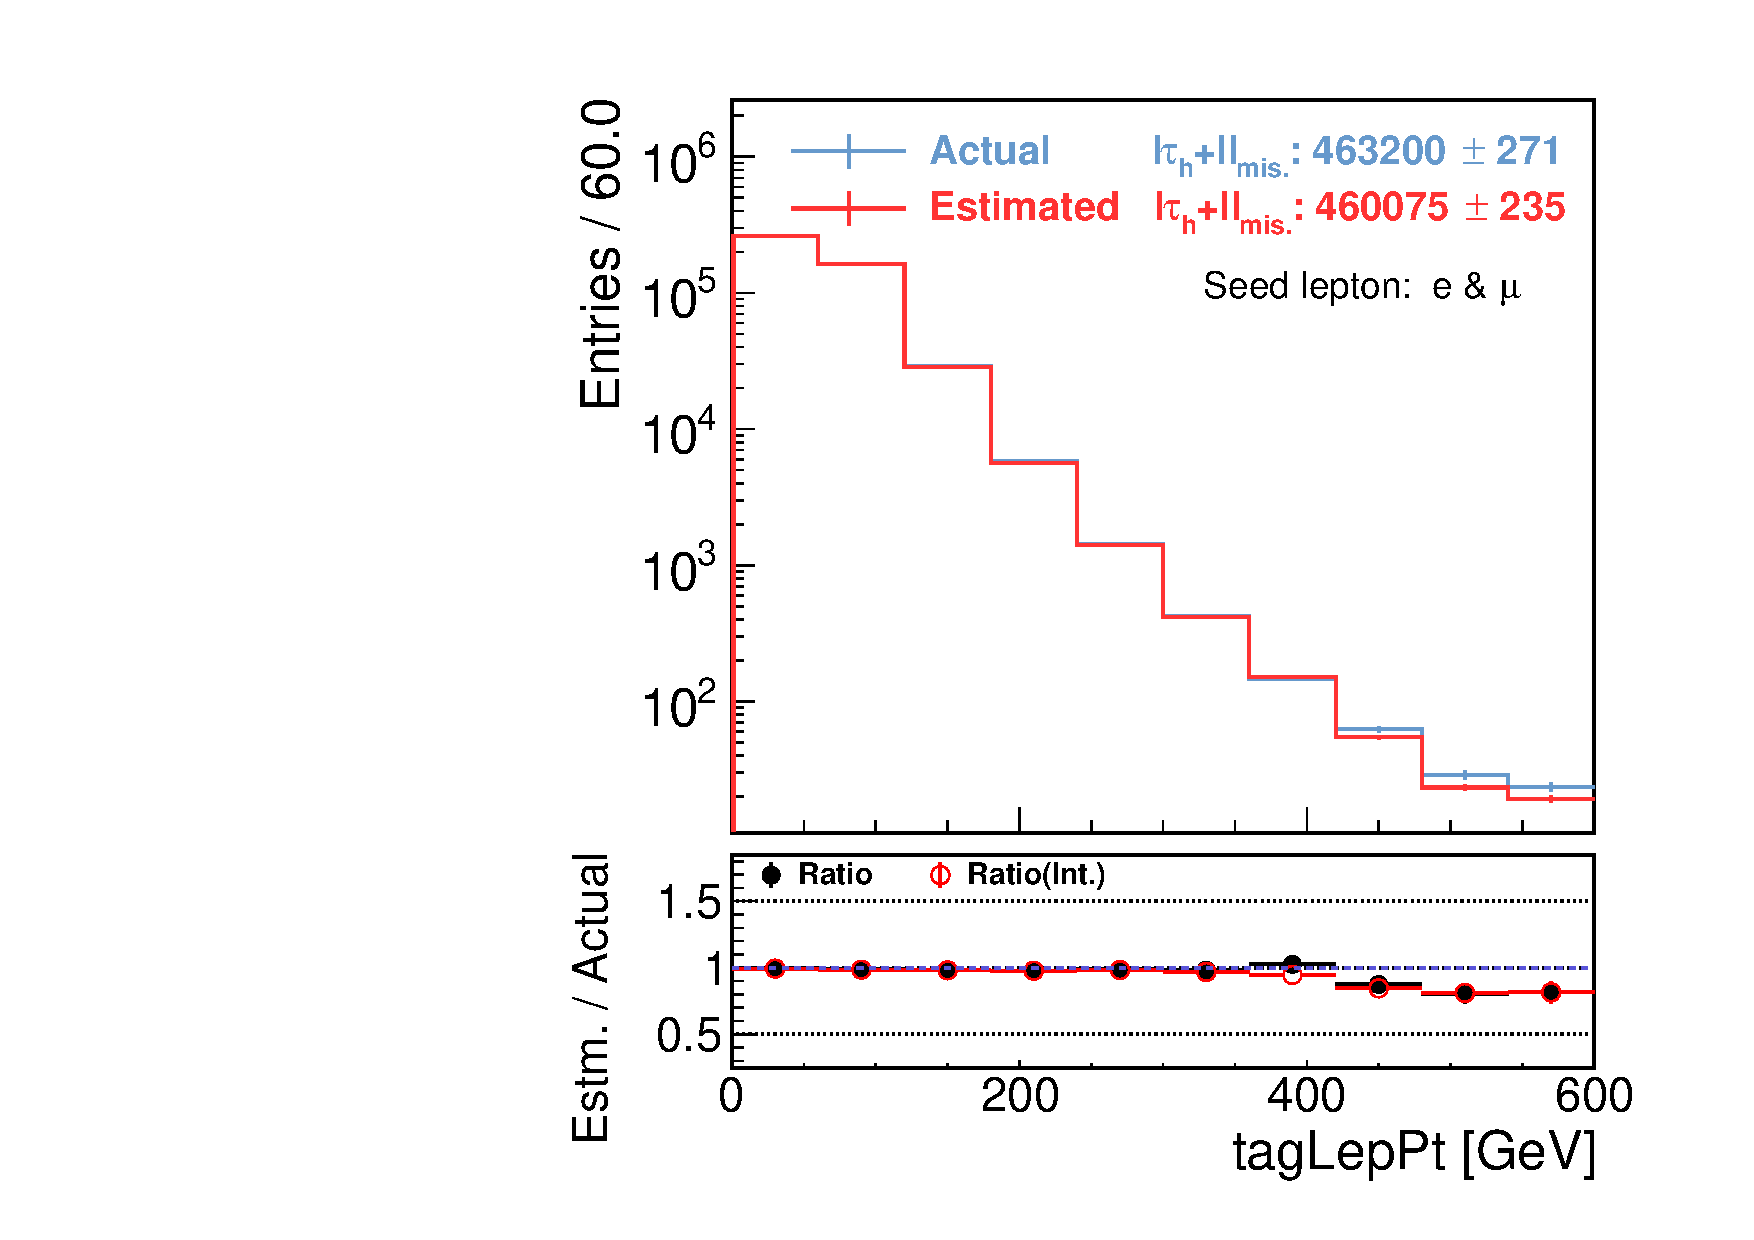
\includegraphics[width=0.32\textwidth]{figures/BGestimation/ObjReplacement/mcClosure/All_emu/All_emu_tagLepPt__trMode4_NoSys.pdf}}
    \subfigure[]{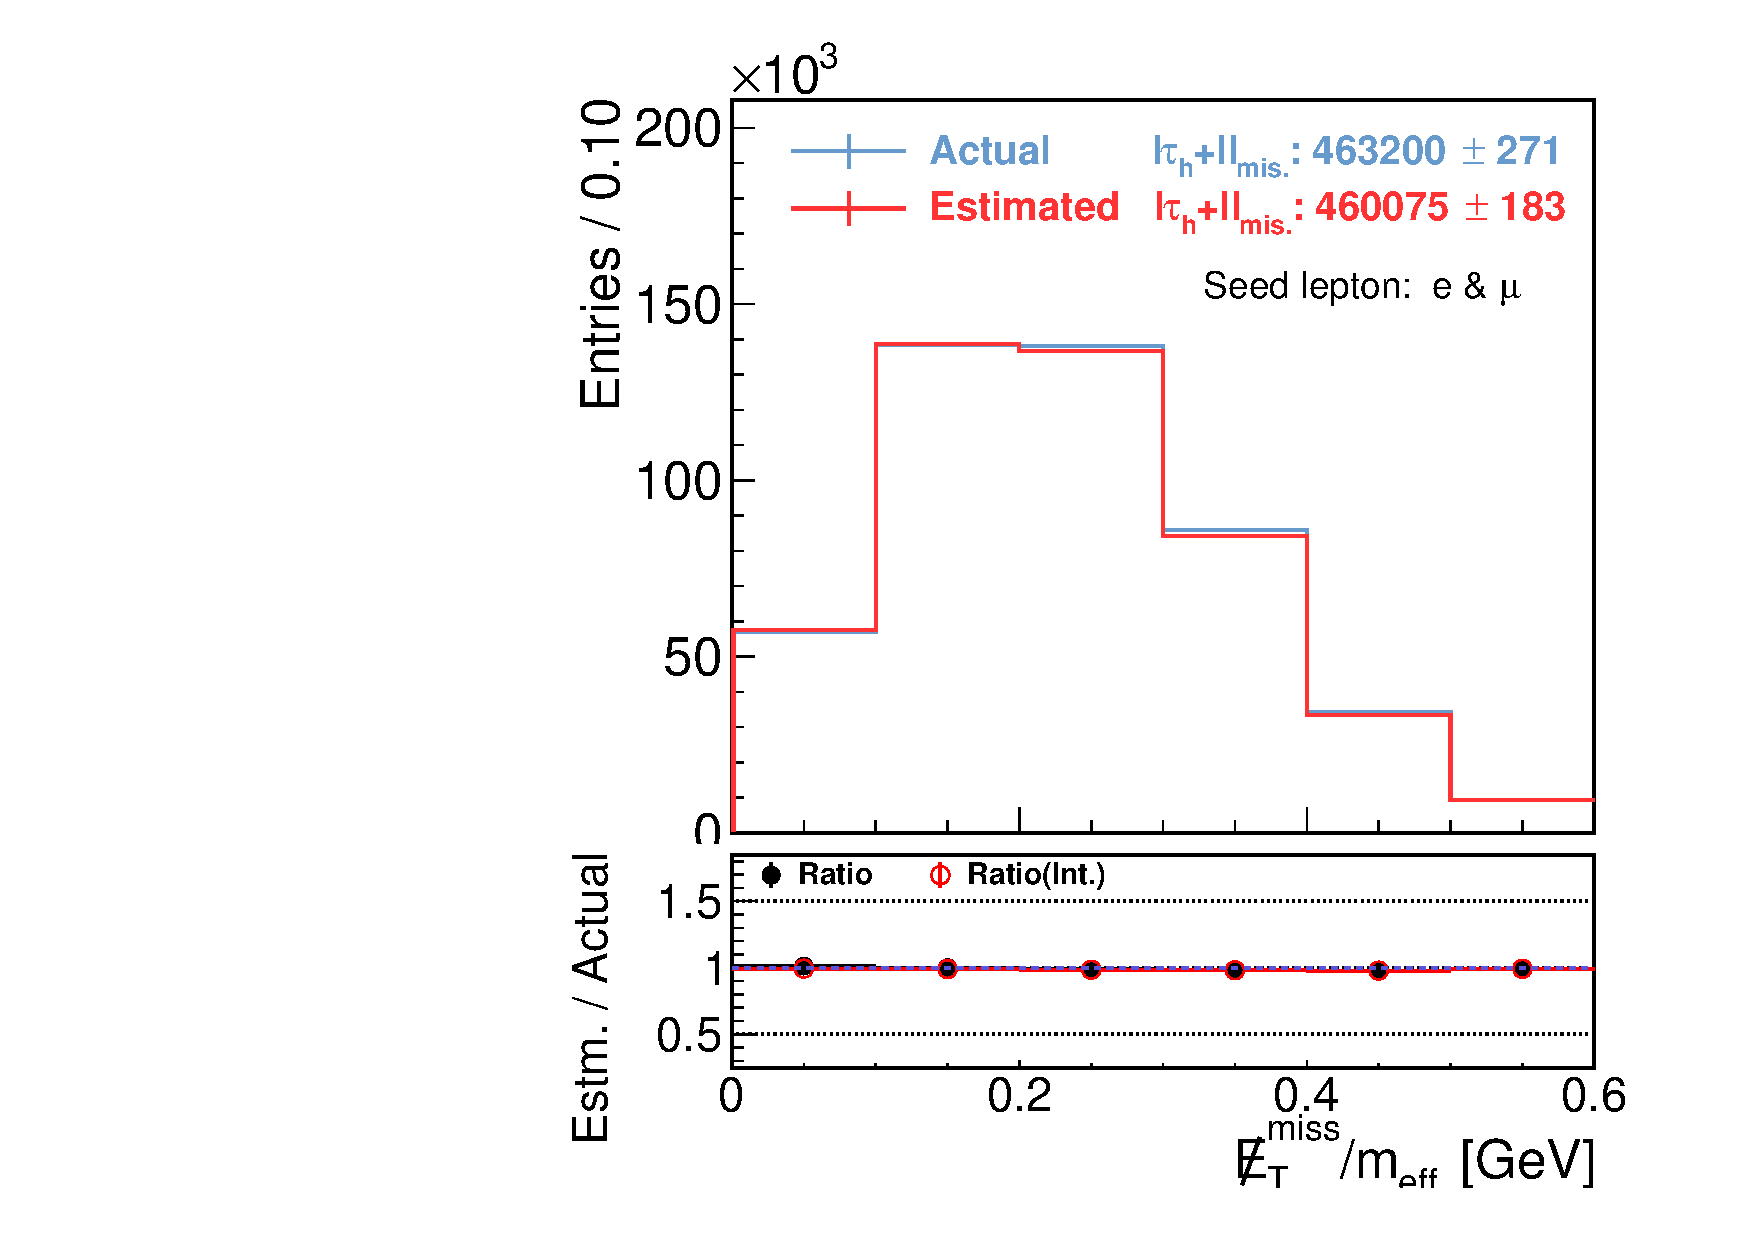
\includegraphics[width=0.32\textwidth]{figures/BGestimation/ObjReplacement/mcClosure/All_emu/All_emu_metOverMeff__trMode4_NoSys.pdf}}
    \subfigure[]{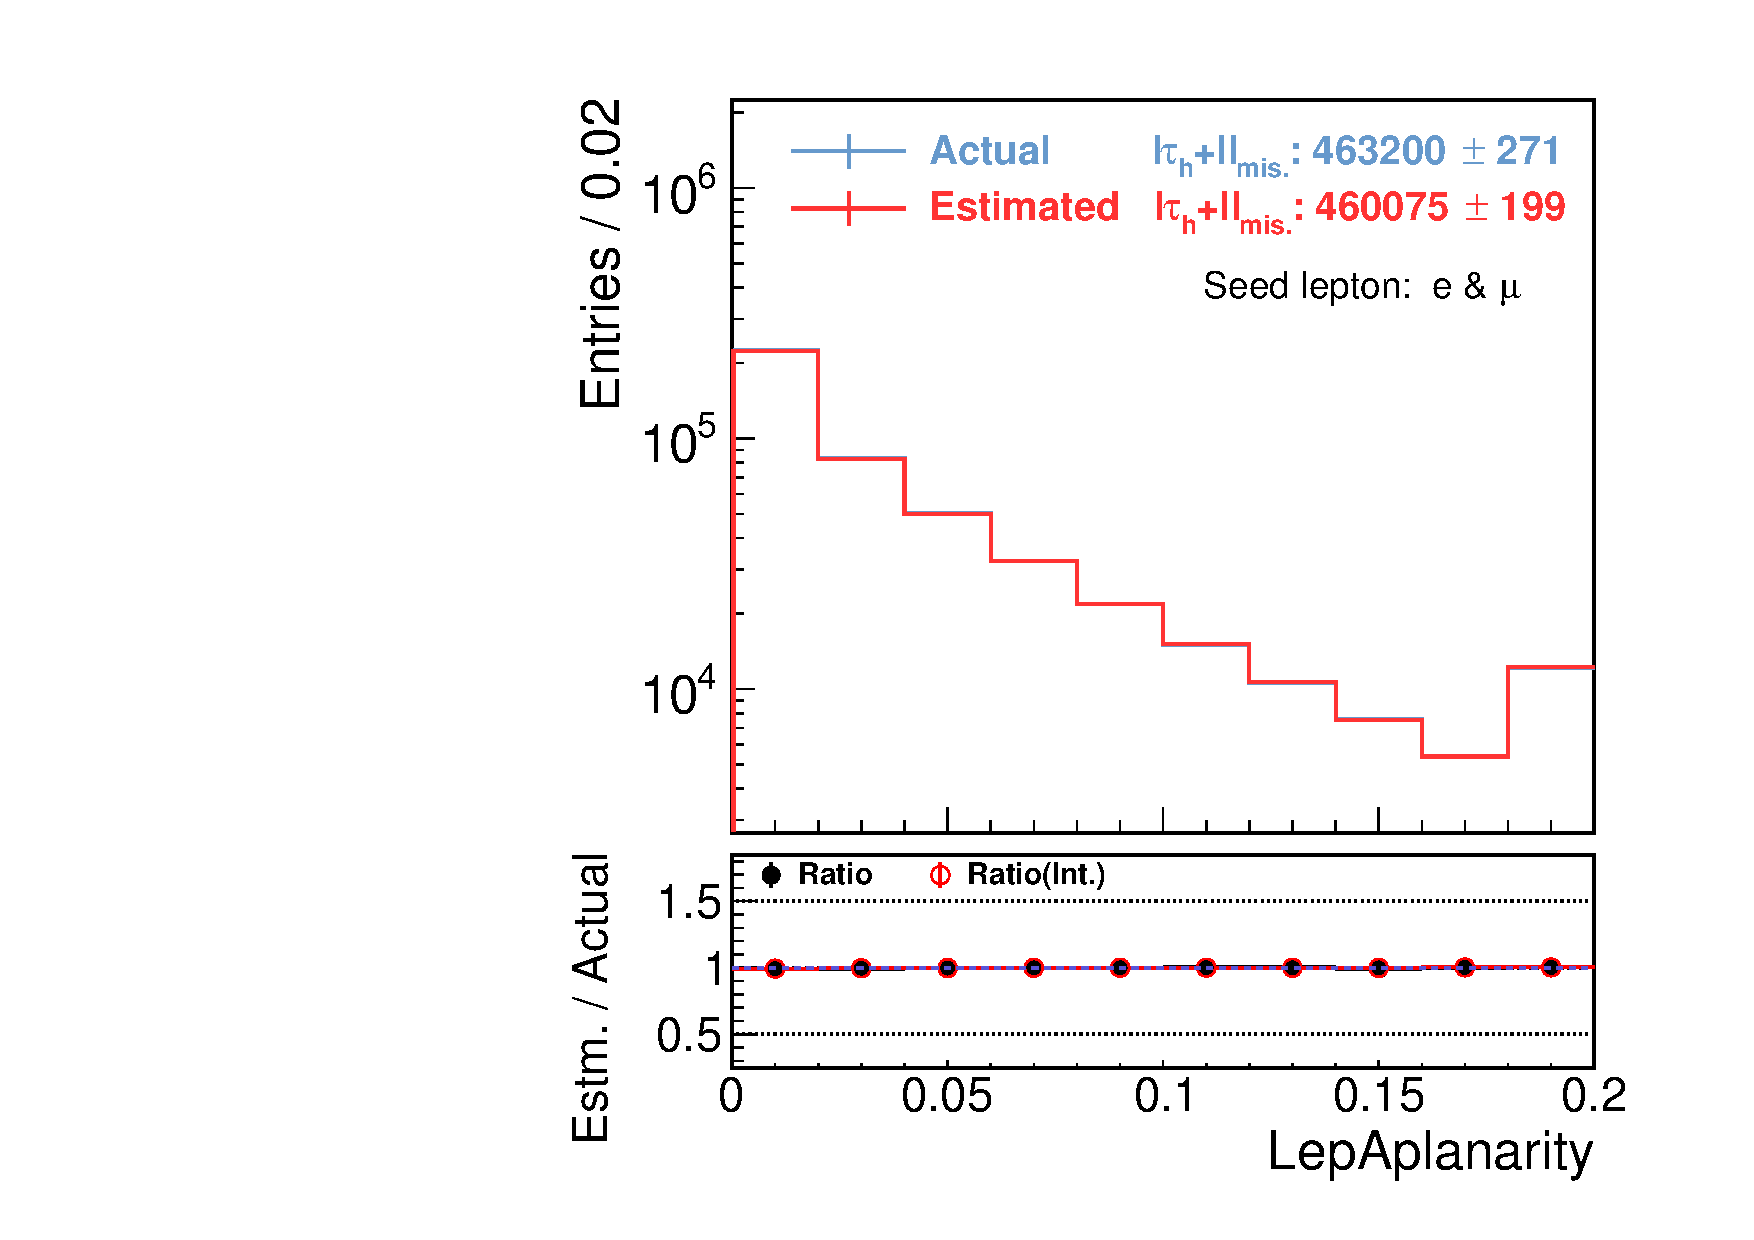
\includegraphics[width=0.32\textwidth]{figures/BGestimation/ObjReplacement/mcClosure/All_emu/All_emu_LepAplanarity__trMode4_NoSys.pdf}}
    \subfigure[]{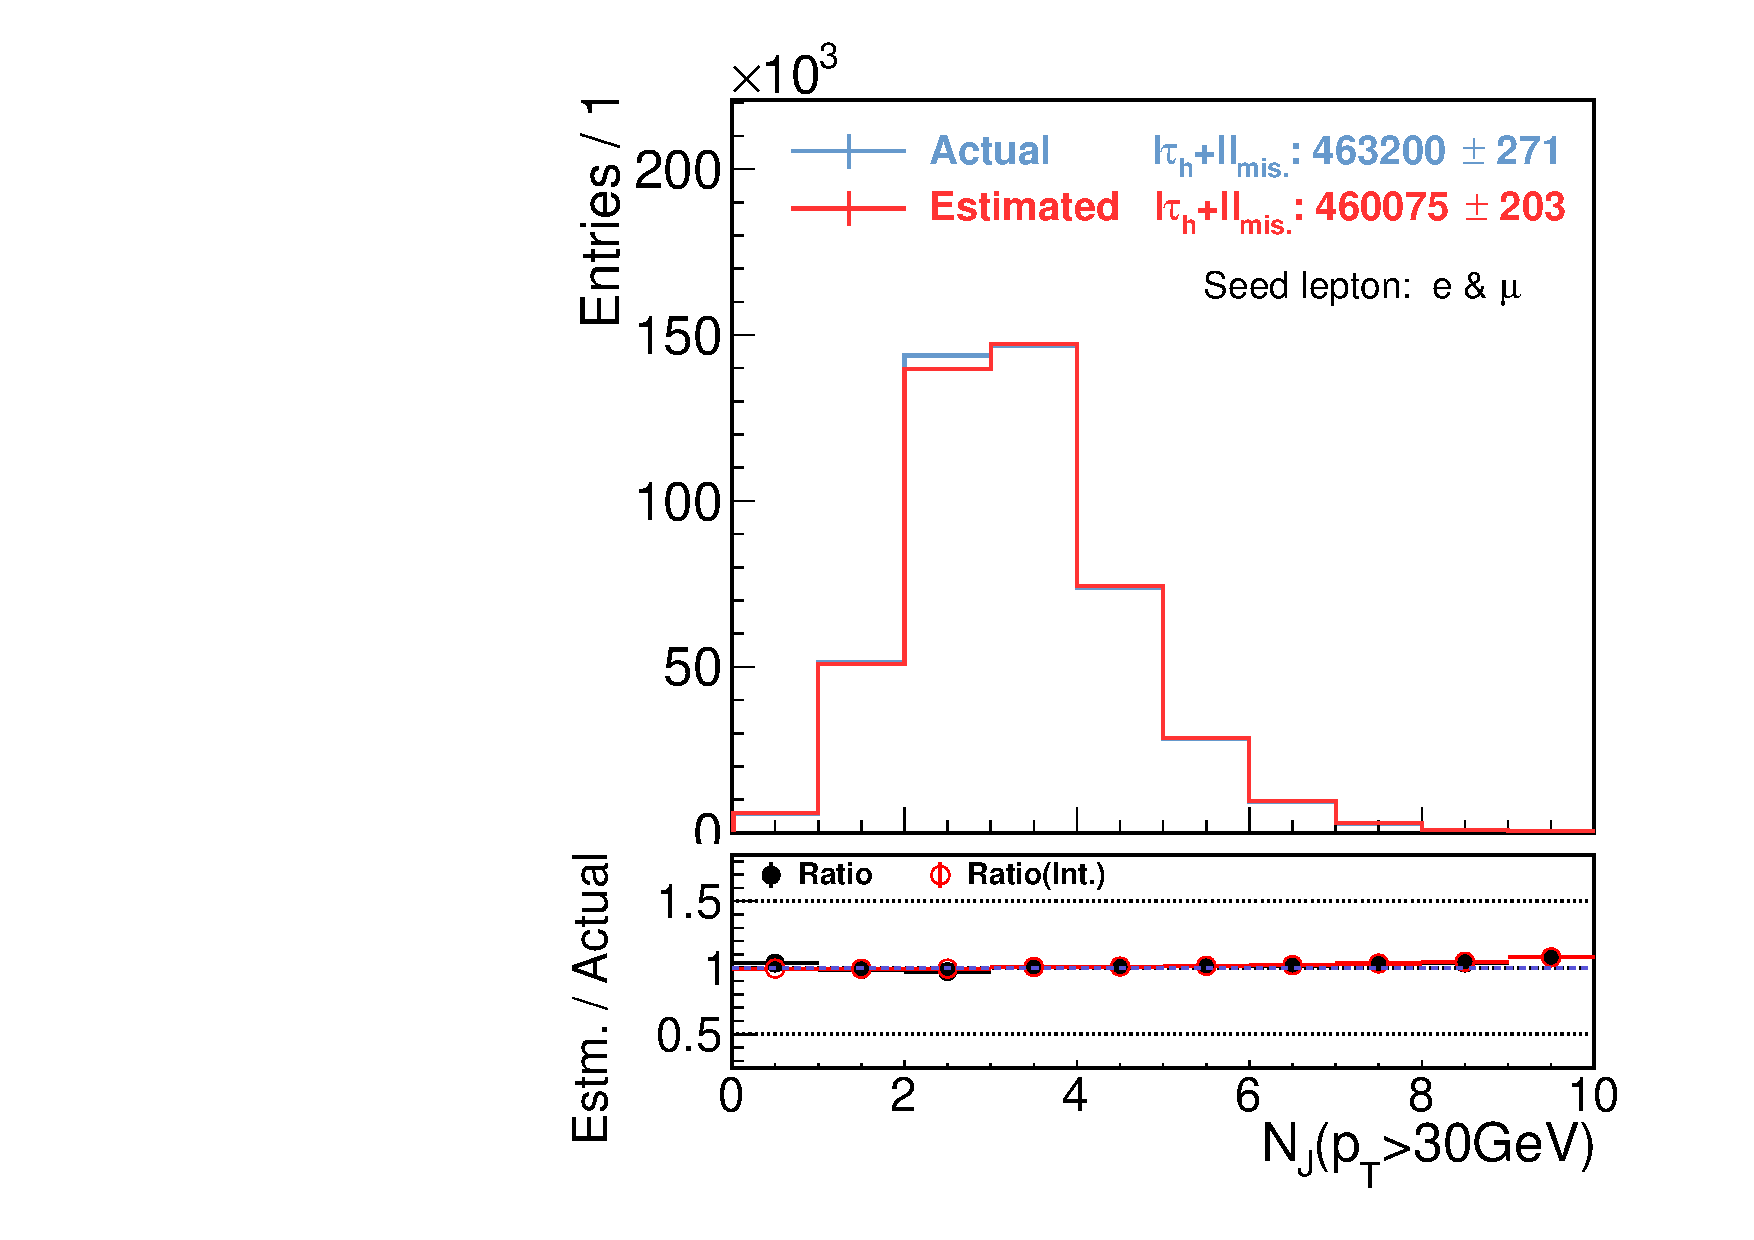
\includegraphics[width=0.32\textwidth]{figures/BGestimation/ObjReplacement/mcClosure/All_emu/All_emu_nJet30__trMode4_NoSys.pdf}}
    \subfigure[]{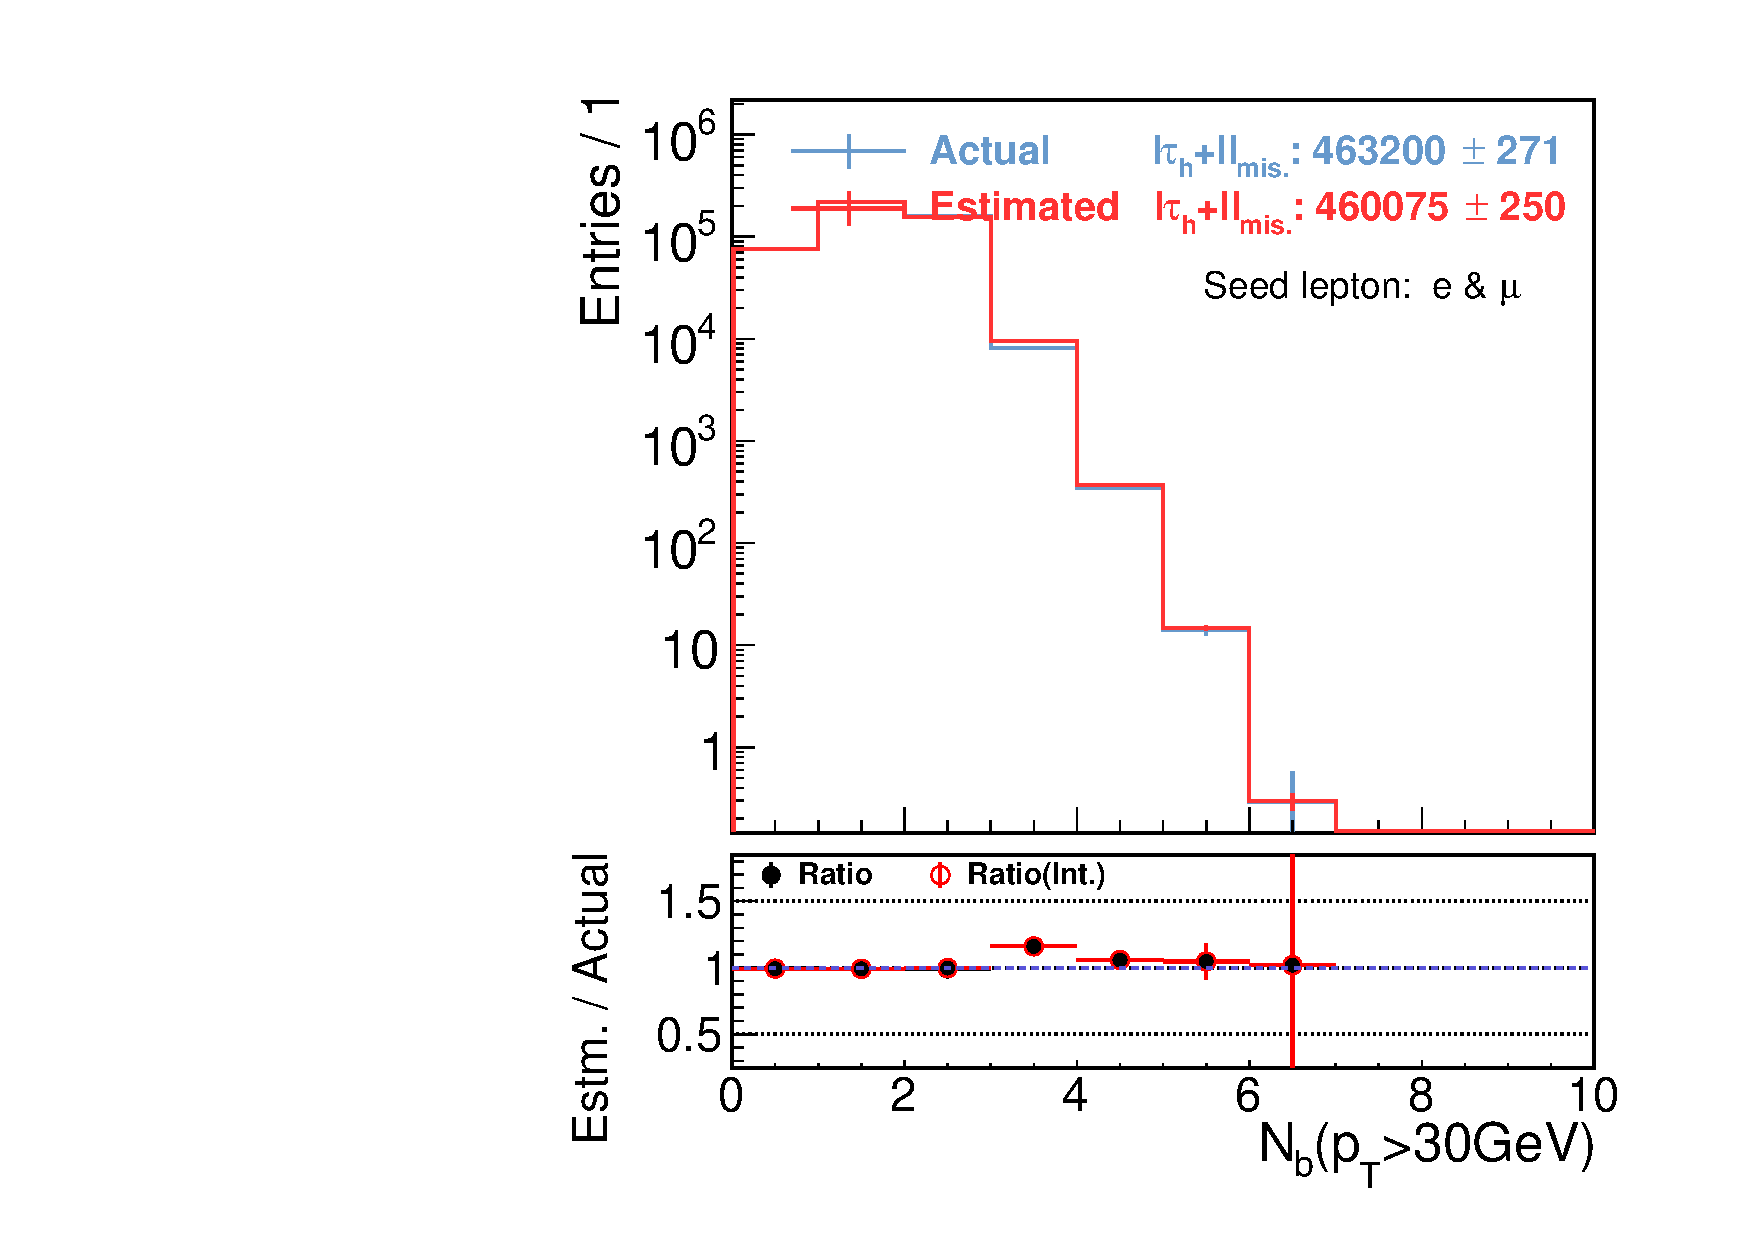
\includegraphics[width=0.32\textwidth]{figures/BGestimation/ObjReplacement/mcClosure/All_emu/All_emu_nBJet30__trMode4_NoSys.pdf}}
    \caption{ MC closure test for \textbf{combined estimation of missing lepton rep. and tau rep.} using $t\bar{t}$ MC sample. Seed events are collected by the single-lepton trigger. $p_T>35\gev$ for the leading lepton is required. \textbf{Both electrons and muons in the seed events are replaced}. Red points in the bottom plots show the ratio of integrated yields for the two histograms above the x-position that the point indicates. \label{fig::ObjReplace::mcClosure_All_emu} }
\end{figure}
 %%%%%%%%%%%%%%%%%%%%%%%%%%

